\documentclass[landscape]{foils} 
\newif\ifpdf
\ifx\pdfoutput\undefined
\pdffalse % we are not running PDFLaTeX
\else
\pdfoutput=1 % we are running PDFLaTeX
\pdftrue
\fi

\ifpdf
\usepackage[pdftex]{graphicx}
\else
\usepackage{graphicx}
\fi

\ifpdf
\DeclareGraphicsExtensions{.pdf, .jpg, .tif, .png}
\else
\DeclareGraphicsExtensions{.eps, .jpg}
\fi

%\usepackage{pslatex}
\usepackage{tabularx,dcolumn, graphicx, amsfonts,amsmath}  
\usepackage[sectionbib]{natbib}
\bibliographystyle{apalike}
\usepackage{picinpar}
\usepackage{multirow}
\usepackage{rotating}
\usepackage{paralist} %compactenum
\setlength{\voffset}{-0.5in}
%\setlength{\hoffset}{-0.5in}
%\setlength{\textwidth}{10.5in}
\setlength{\textheight}{7in}
\setlength{\parindent}{0pt}
%\pagestyle{empty}
%\renewcommand{\baselinestretch}{2.0}
\DeclareMathSymbol{\expect}{\mathalpha}{AMSb}{'105}
\def\p{\rm p}
\def\pp{\rm P}
% this are commands that come with the color package
\usepackage{color}
\usepackage{fancyhdr}


\pagestyle{empty}
%define colors
\definecolor{mediumblue}{rgb}{0.0509,0.35,0.568}
\definecolor{blue}{rgb}{0.0109,0.15,0.468}
\definecolor{black}{rgb}{0.04,0.06,0.2}
\definecolor{darkblue}{rgb}{0.03,0.1,0.2}
\definecolor{darkgreen}{rgb}{0.03,0.5,0.2}
\definecolor{lightblue}{rgb}{0.85,0.9333,0.95}
\definecolor{lightblue2}{rgb}{0.270588, 0.45098, 0.701961}
\definecolor{white}{rgb}{1.0,1.0,1.0}
\definecolor{yellow}{rgb}{0.961,0.972,0.047}
\definecolor{red}{rgb}{0.9,0.1,0.1}
\definecolor{orange}{rgb}{1.0,0.4,0.0}
\definecolor{grey}{rgb}{0.5,0.5,0.5}
\definecolor{violet}{rgb}{0.619608, 0.286275, 0.631373}
\definecolor{mybackgroundcolor}{rgb}{1.0,1.0,1.0}

%\definecolor{light}{rgb}{.5,0.5,0.0}
\definecolor{light}{rgb}{.3,0.3,0.3}

% sets backgroundcolor for whole document 
\pagecolor{mybackgroundcolor}
% sets text color
%\color{black}
% see below for an example how to change just a few words
% using \textcolor{color}{text}

\font \courier=pcrb scaled 2000
\newcommand{\notetoself}[1]{{\textsf{\textsc{\color{red} #1}}}\\}

\newcommand{\answer}[1]{{\sf \color{red} #1}}

\usepackage{pdfpages}
 
\newcommand{\section}{\secdef \newsection\newsection}
%\renewcommand{\labelitemi}{\includegraphics[width=5mm]{images/bullet.pdf}}
\newcommand{\newsection}[1]{%
{
	\par\flushleft\large\sf\bfseries \vskip -2cm #1\\\rule[0.7\baselineskip]{\textwidth}{0.5mm}\par}}

\newcommand{\subsection}{\secdef \test\test}
\newcommand{\test}[1]{%
	{\par\flushleft\normalsize\sf\bfseries #1: }}
\newcommand{\M}{\mathcal{M}}
\newcommand{\prob}{{\rm Prob~}}
\def\showy#1{{\normalsize\sf\bfseries #1}}
\def\donotuse#1{}

\newcommand{\entrylabel}[1]{\mbox{#1}\hfil}
\newenvironment{entry}
	{\begin{list}{}%
		{\renewcommand{\makelabel}{\entrylabel}%
		\setlength{\labelwidth}{35pt}%
		\setlength{\leftmargin}{\labelwidth+\labelsep}%
	}%
	{\end{list}}}

\newcommand{\poltext}{{\copyright\ 2002--2010 by Paul O. Lewis -- Modified by  Mark Holder with permission from Paul Lewis}}

\newcommand{\pol}{{\footnotesize \poltext}}
\newcommand{\myBackground}{\begin{picture}(0,0)(0,0)  \put(-40,-70){\makebox(0,0)[l]{\includegraphics[width=33cm]{images/baby_blue.jpg}}} \end{picture}}
\newcommand{\myFooter}{}
%\begin{picture}(0,0)(0,0)
%	\put(0,-185){\pol}
%\end{picture}}
\newcommand{\myNewSlide}{\newpage\myFooter} % \myBackground}

\usepackage{bm}
\usepackage{mathrsfs}
\usepackage{url}
\usepackage{hyperref}
\hypersetup{backref,  linkcolor=blue, citecolor=black, colorlinks=true, hyperindex=true}

\usepackage{pdfpages}
\usepackage{bm}

\begin{document}

\myNewSlide
\huge 
{\begin{center}Hypothesis testing and phylogenetics\end{center}}
\vskip 3cm
\large Woods Hole Workshop on Molecular Evolution, 2017\par 
\vskip 3cm
\normalsize
\normalsize
Mark T. Holder\\
University of Kansas\par 
\vskip 1cm
Thanks to Paul Lewis, Joe Felsenstein, and Peter Beerli for slides.

\myNewSlide
\section*{Motivation}
Pipeline of:\par
Data collection $\rightarrow$ Alignment $\rightarrow$ Model selction $\rightarrow$ Tree estimation

gives us a {\em point estimate} of the best tree.

This lecture/lab covers:
\begin{compactenum}
	\item How confident should we be that this tree is correct?
	\item Can we be confident in some aspects of the tree ({\em e.g.} some clades)?
	\item If our question of interest is about evolution of characters, can
		we answer that question despite our uncertainty about the tree?
\end{compactenum}



%\myNewSlide
\section*{Conclusions 1 - confidence on trees}\large
\large
\begin{compactenum}
    \item Non-parametric bootstrapping: useful for assessing sampling error, but a little hard to interpret  precisely.
    \begin{compactitem}
        \item Susko's  aBP gives $1 - aBP\approx P$-value for the hypothesis that a recovered branch is not present in the true tree. 
    \end{compactitem}
    \item ``How should we assign a $P$-value to tree hypothesis?'' is surprisingly complicated.
    \begin{compactitem}
        \item Kishino-Hasegawa (KH-Test) if testing 2 ({\em a priori}) trees.
        \item Shimodaira's approximately unbiased (AU-Test) for sets of trees.
        \item Parametric bootstrapping (can simulate under complex models)
    \end{compactitem}
\end{compactenum}

\myNewSlide
\section*{Conclusions 2 - confidence about evo.~hypotheses}
If $H_0$ is about the evolution of a trait:
\begin{compactenum}
    \item $P$-value must consider uncertainty of the tree:
    \begin{compactitem}
        \item can be large $P$ over confidence set of trees.
        \item Bayesian methods (covered tomorrow) enable prior predictive or posterior predictive $P$-values.
    \end{compactitem}
\end{compactenum}

\myNewSlide
\section*{Conclusions 3 - simulate your own null distributions}
(the focus of the lab)
\begin{compactenum}
    \item In phylogenetics we often have to simulate data to approximate $P$-values 
    \item Designing the simulations requires care to make a convincing argument.
\end{compactenum}

%\myNewSlide
\section*{Reasons phylogenetic inference might be wrong}
\Large
\begin{compactenum}
    \item {\em Systematic error} -- Our inference method might not be sophisticated enough
    \item \underline{{\em Random error}} -- We might not have enough data --  we are misled by sampling error.
\end{compactenum}

\myNewSlide
\begin{picture}(0,0)(0,0)
      \put(-60,-280){\makebox(0,0)[l]{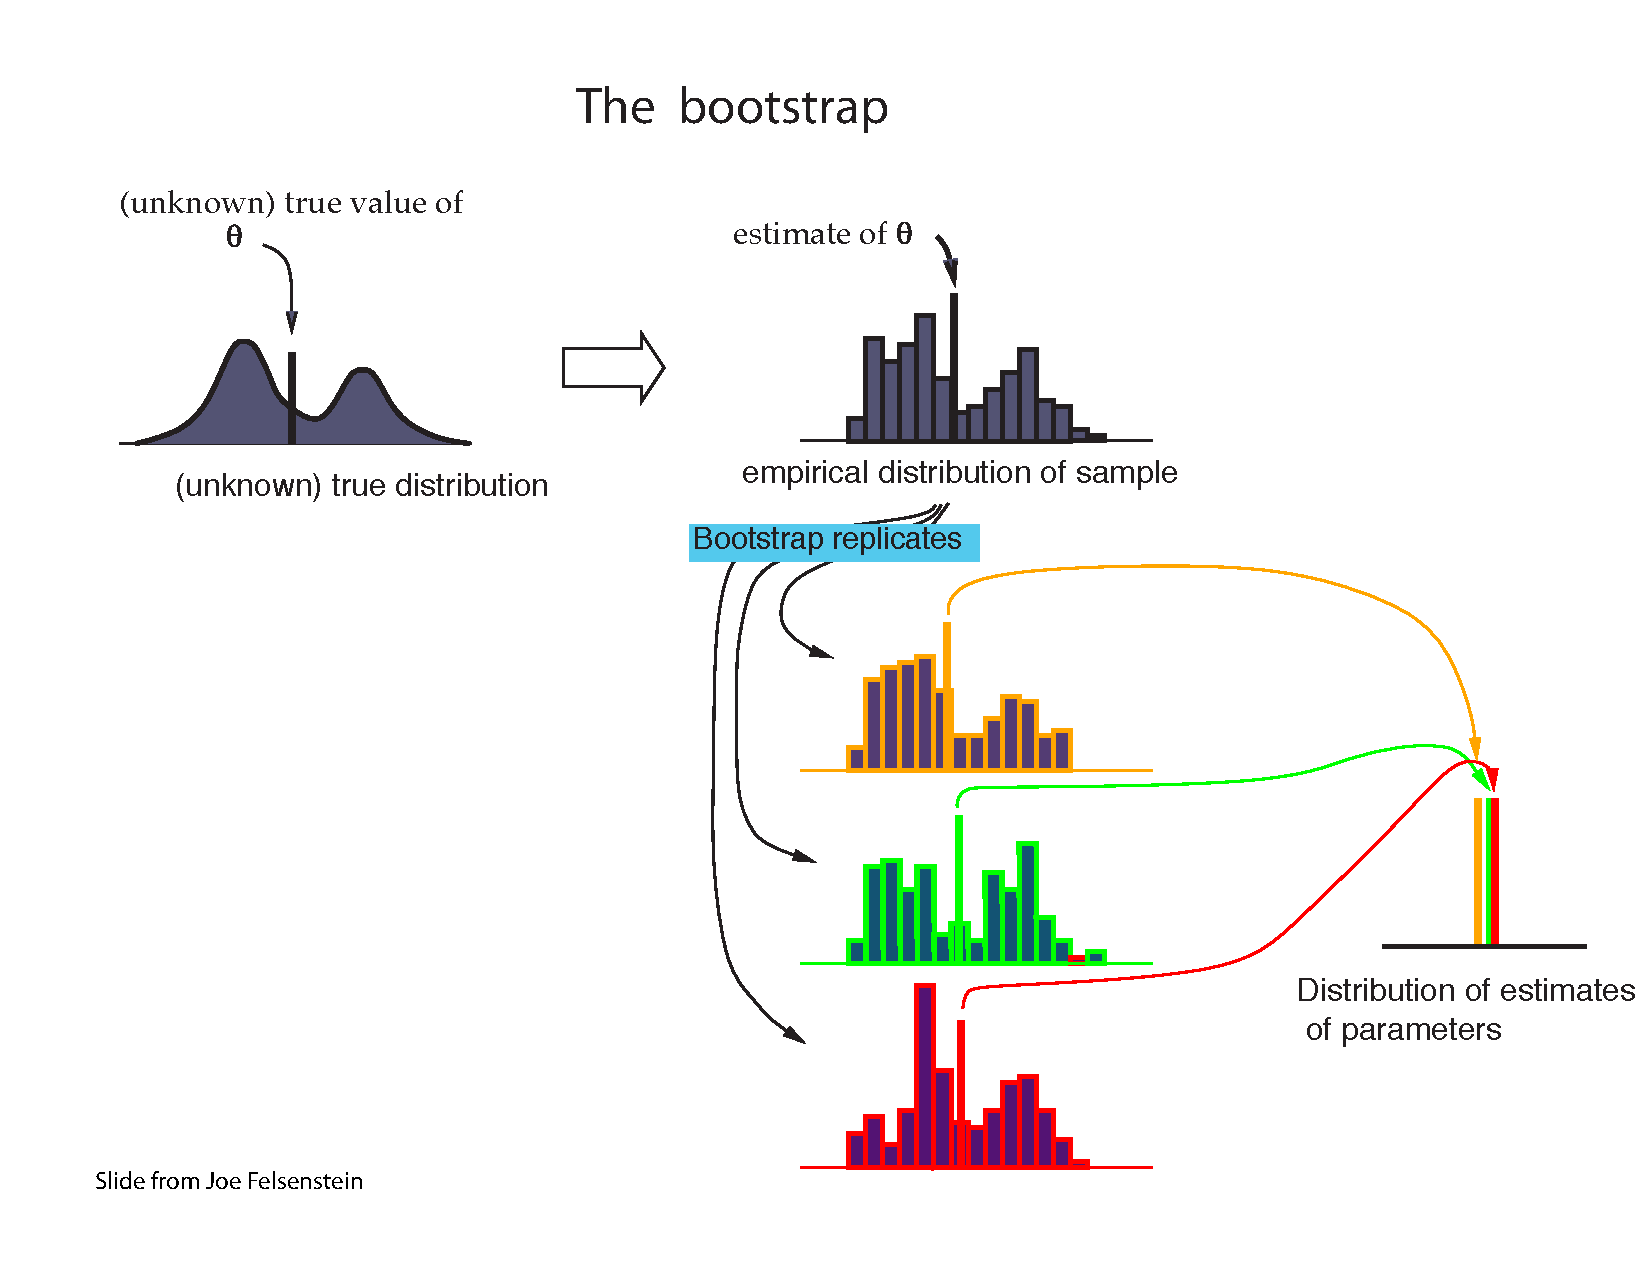
\includegraphics[scale=1.2]{../newimages/JoeFelsBootFig1.pdf}}}
      \put(0,-716){\makebox(0,0)[l]{
\includegraphics[scale=2]{../newimages/whitepage.pdf}}}
\end{picture}

\myNewSlide
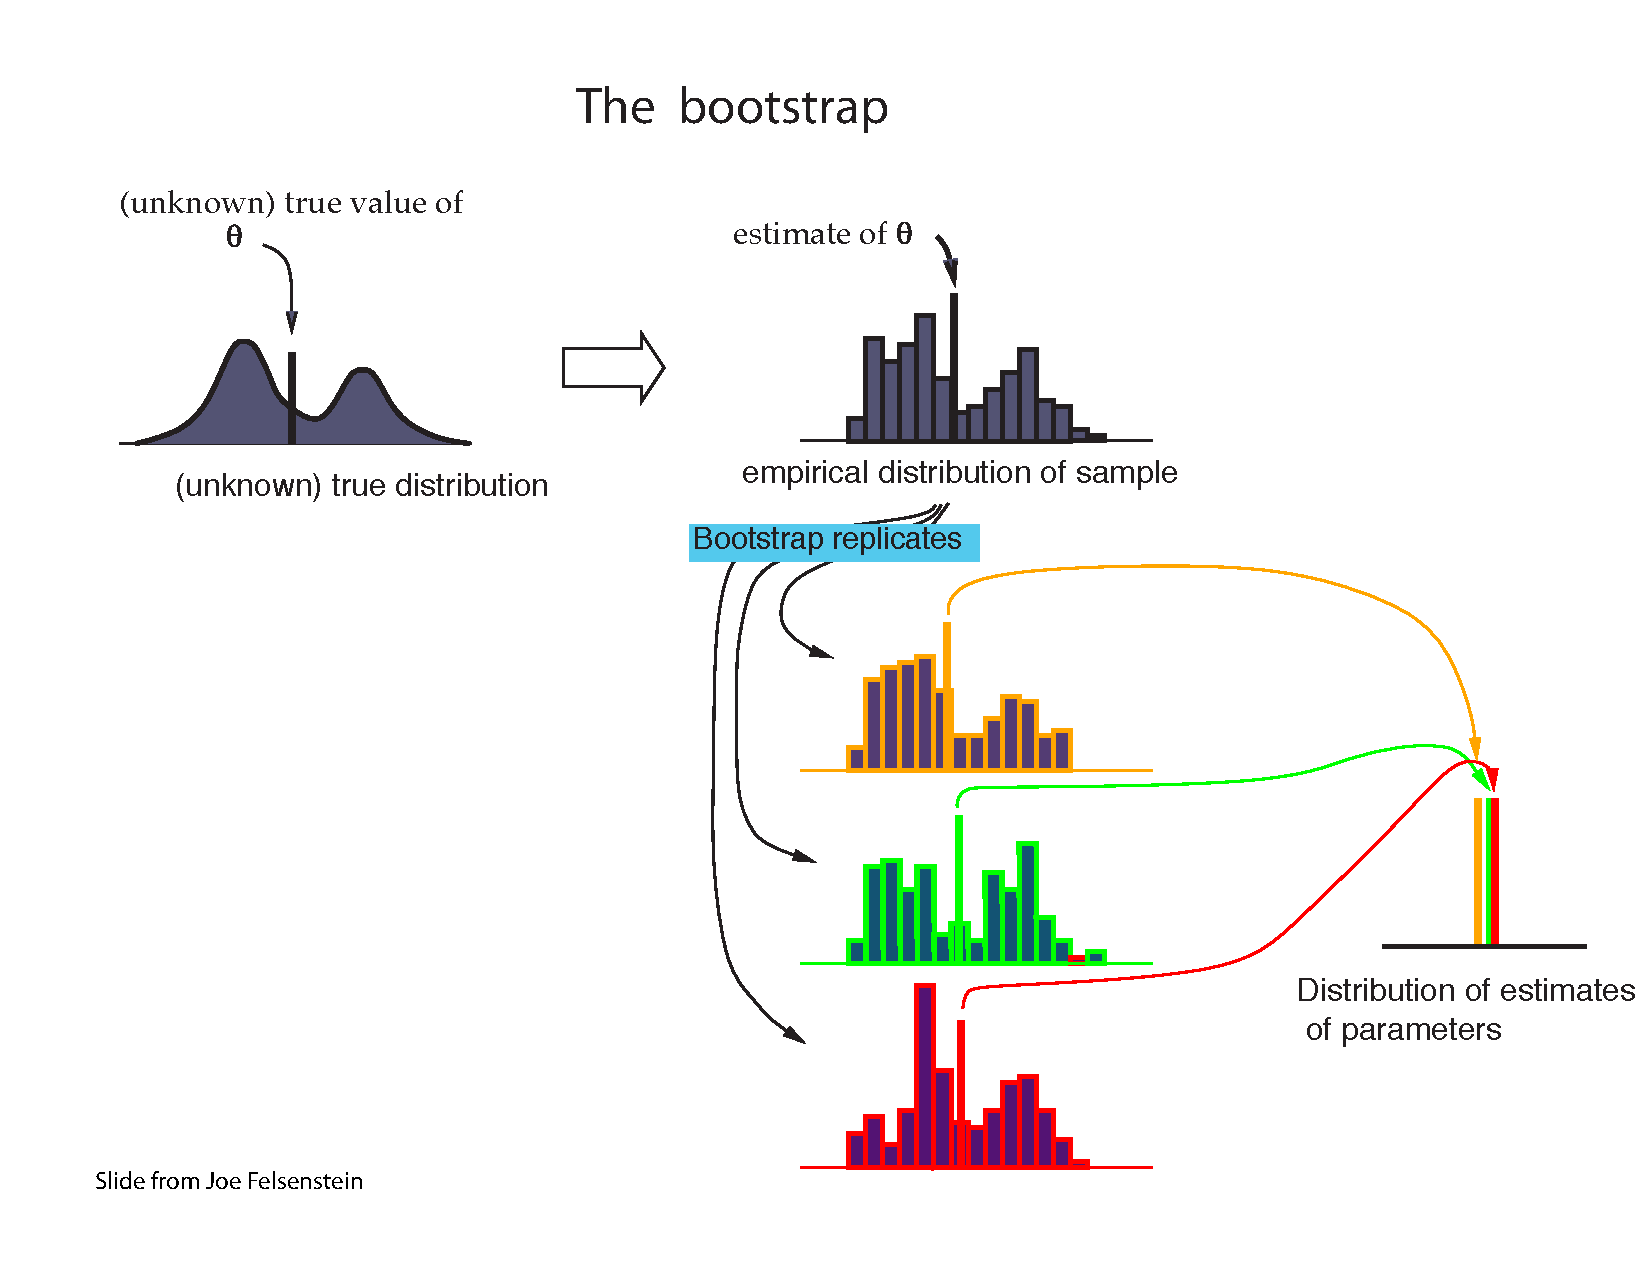
\includepdf[pages={1}]{../newimages/JoeFelsBootFig1.pdf} 

\myNewSlide
\begin{picture}(0,0)(0,0)
      \put(-70,-316){\makebox(0,0)[l]{
\includegraphics[scale=2]{../newimages/greypage.pdf}}}
      \put(-40,-200){\makebox(0,0)[l]{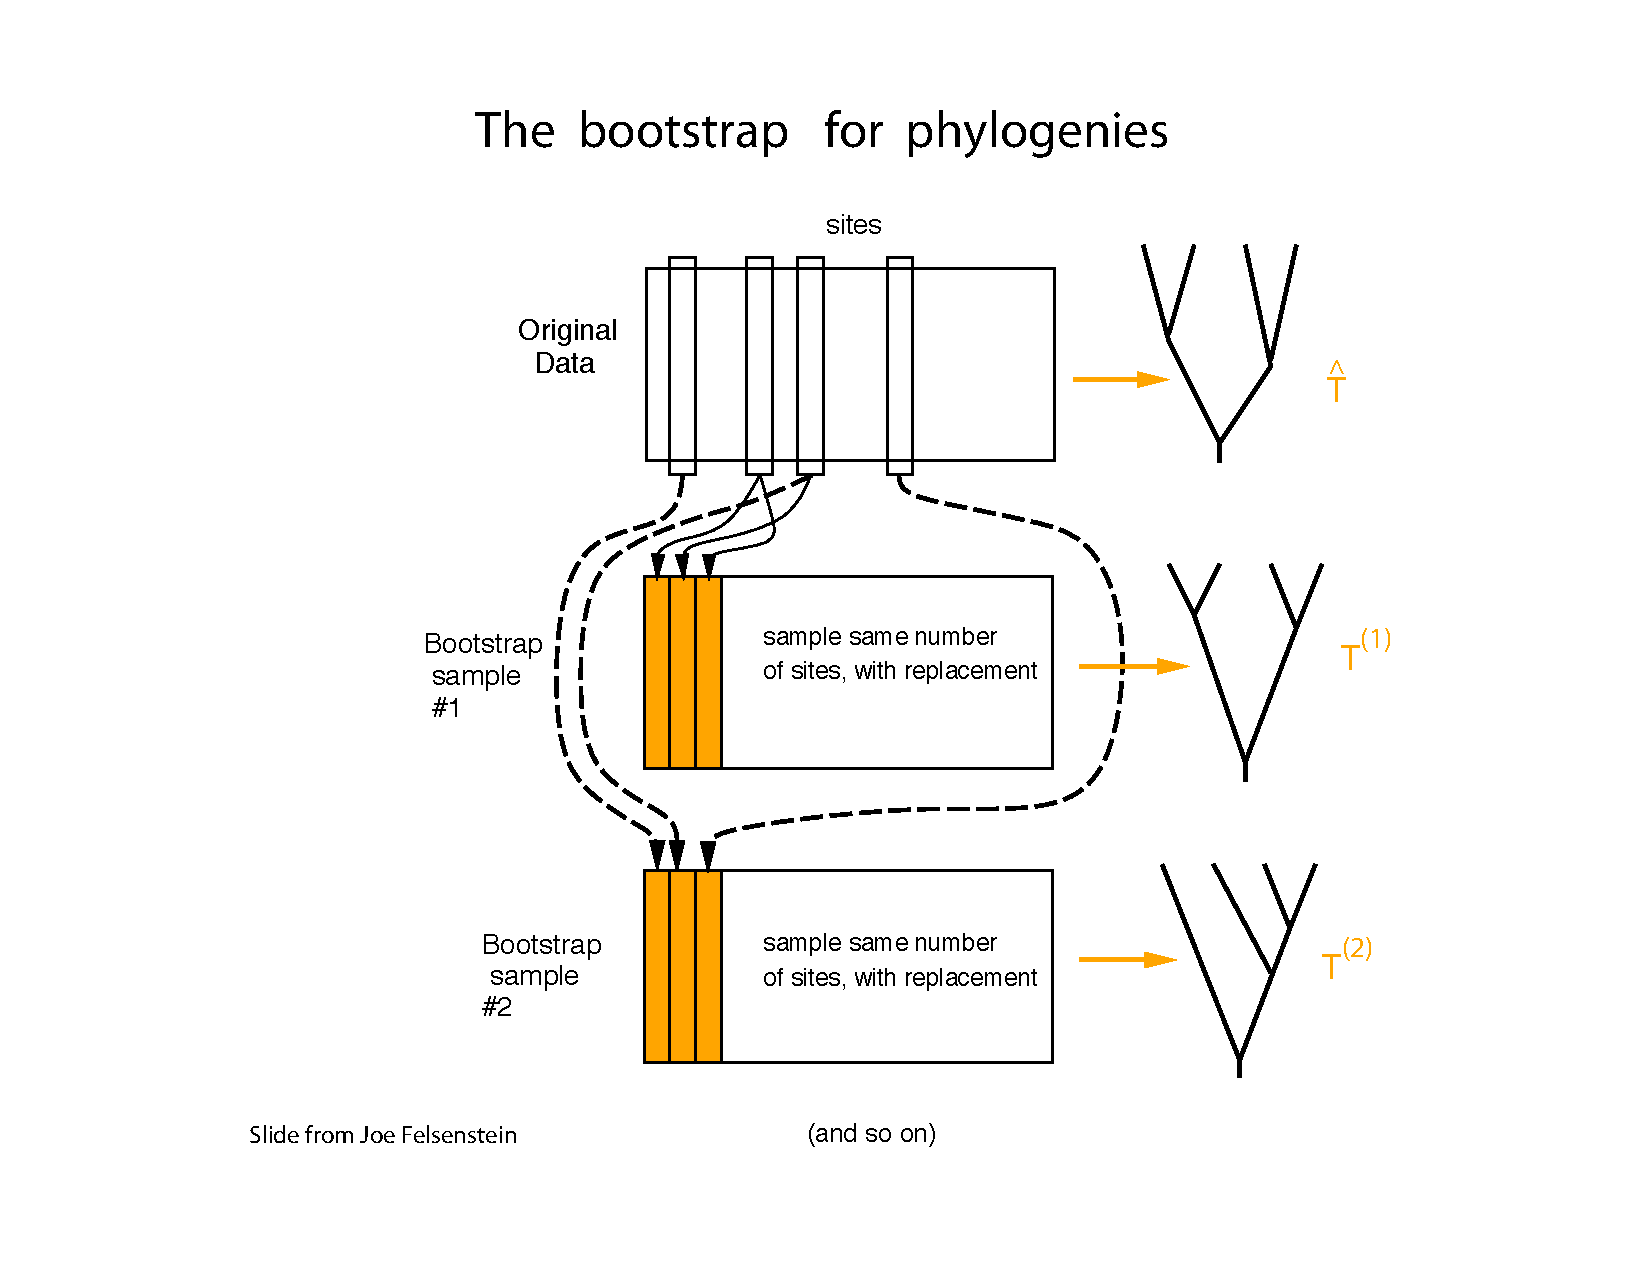
\includegraphics[scale=1.0]{../newimages/JoeFelsBootFig2.pdf}}}
\end{picture}

\myNewSlide
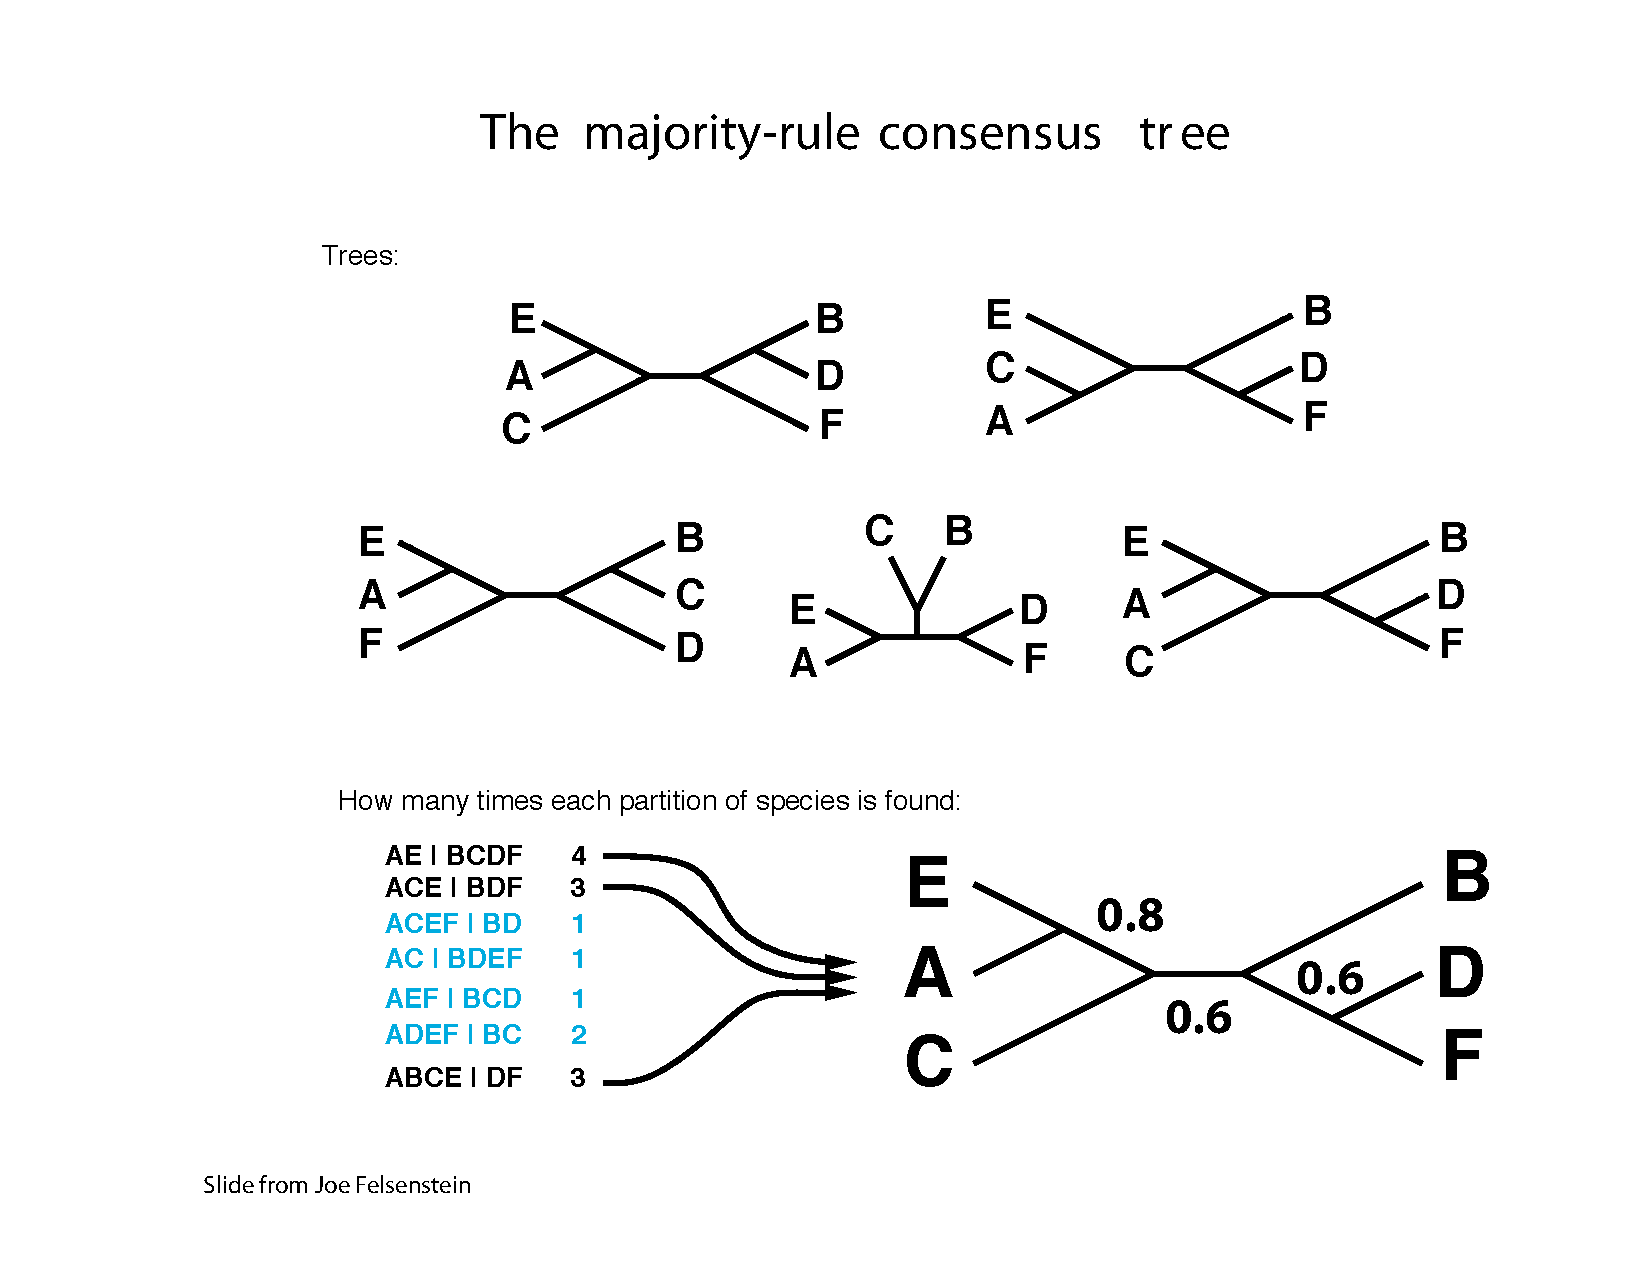
\includepdf[pages={1}]{../newimages/JoeFelsBootFig3.pdf} 



\myNewSlide
\begin{picture}(0,0)(0,0)
      \put(0,-180){\makebox(0,0)[l]{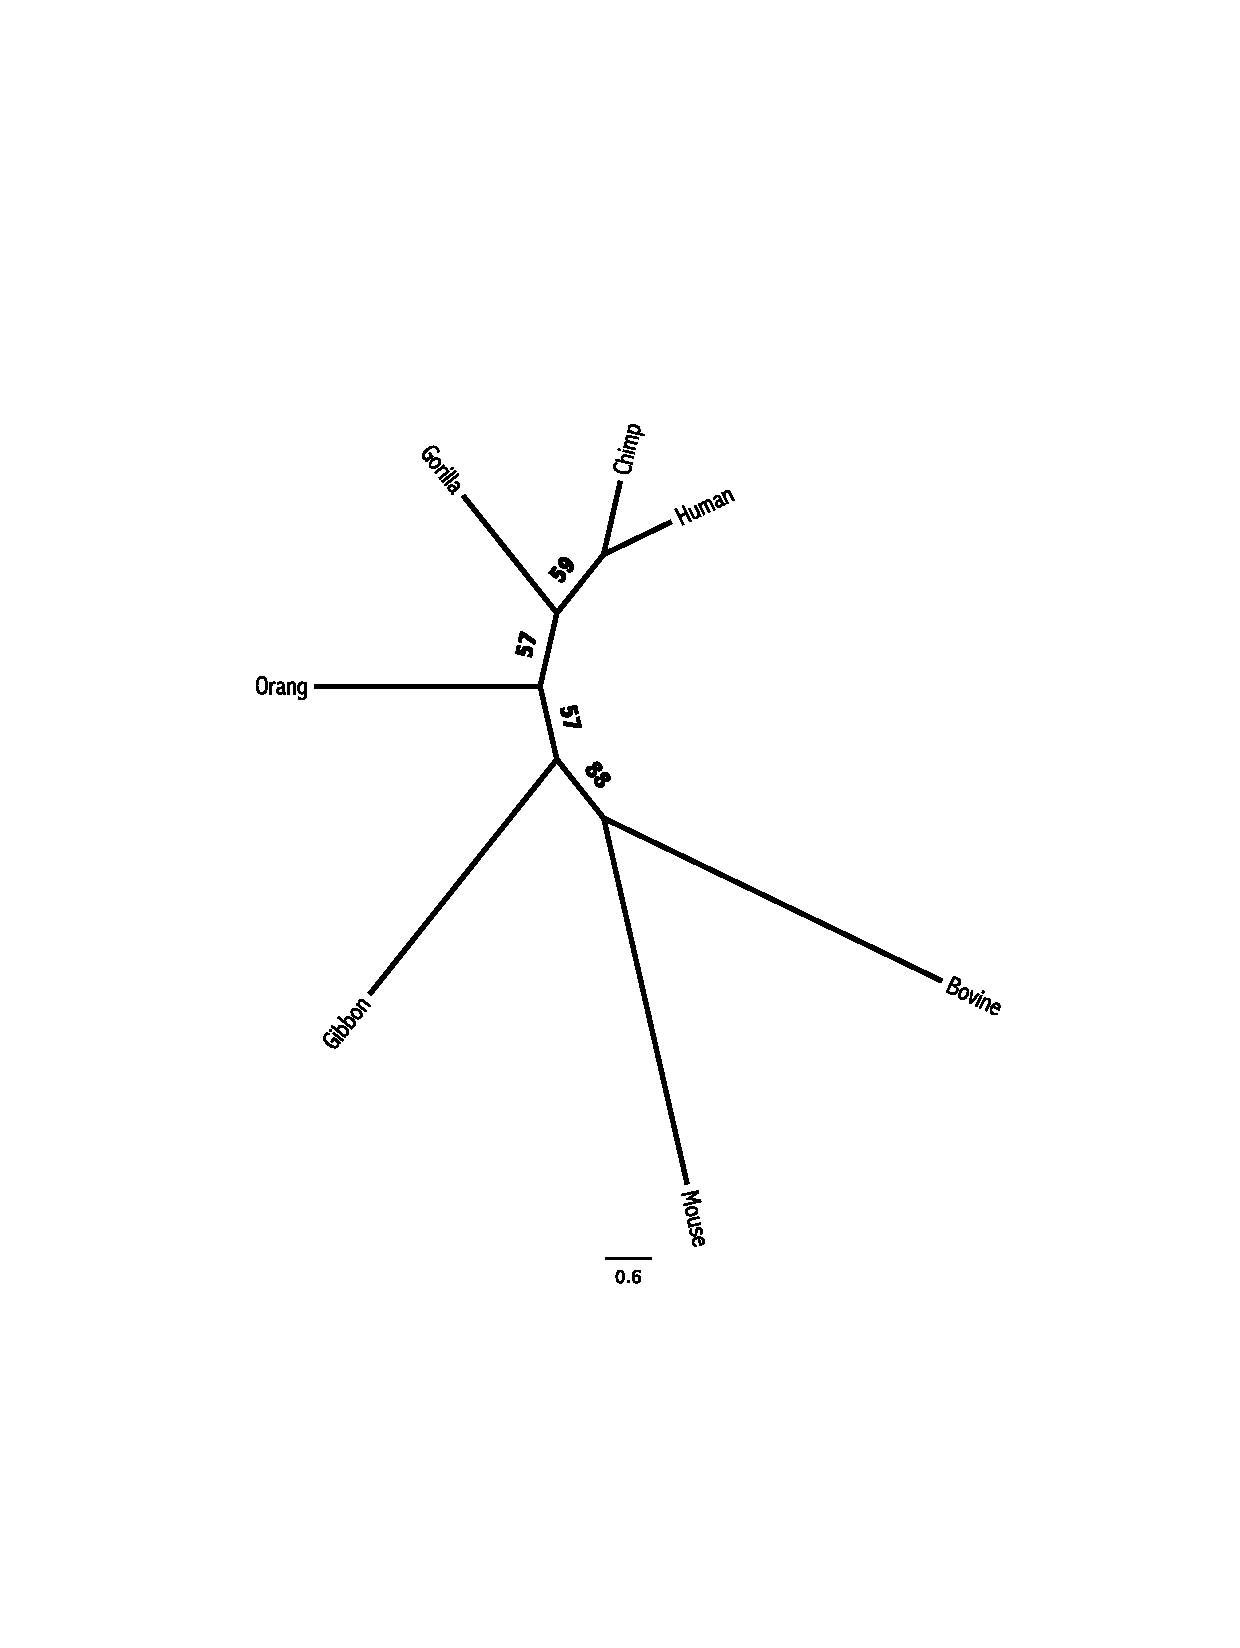
\includegraphics[scale=1.2]{../newimages/hasegawaBootFigTree.pdf}}}
      \put(0,-350){\small From Hasegawa's analysis of 232 sites D-loop}
\end{picture}

\myNewSlide
{\large
\url{http://phylo.bio.ku.edu/mephytis/boot-sample.html}

\url{http://phylo.bio.ku.edu/mephytis/parsimony.html}

\url{http://phylo.bio.ku.edu/mephytis/bootstrap.html}
}
\myNewSlide
\section*{Bootstrapping for branch support}
\large
\begin{itemize}
    \item Typically a few hundred bootstrap, pseudoreplicate datasets are produced.
    \item Less thorough searching is faster, but will usually artificially lower bootstrap proportions (BP). However, \citet{AnisimovaGDDG2011} report that RAxML's rapid bootstrap algorithm may inflate BP.
    \item ``Rogue'' taxa can lower support for many splits -- you do not have to use the majority-rule consensus tree to summarize bootstrap confidence statements.
\end{itemize}





\myNewSlide
\Large
Bootstrap proportions have been characterized as providing:
\begin{compactitem}
    \item a measure of repeatability,
    \item an estimate of the probability that the tree is correct (and bootstrapping has been criticized as being too conservative in this context),
    \item the P-value for a tree or clade
\end{compactitem}



\myNewSlide
\section*{Frequentist hypothesis testing: coin flipping example}
$N=100$ and $h=60$\\
Can we reject the fair coin hypothesis? $H_0:\Pr(\mbox{heads}) = 0.5$

The ``recipe'' is:
\begin{compactenum}
    \item Formulate null ($H_0$) and alternative ($H_A$) hypotheses.
    \item Choose an acceptable Type-I error rate (significance level)
    \item Choose a test statistic: $f_H$= fraction of heads in sample. $f_H=0.6$
    \item Characterize the null distribution of the test statistic 
    \item Calculate the $P$-value: The probability of a test statistic value more extreme than $f_H$ arising {\em even if $H_0$  is true}.
    \item Reject $H_0$ if $P$-value is $\leq$ your Type I error rate.
\end{compactenum}

\myNewSlide
\begin{picture}(500,0)(0,0)
      \put(0,-190){\makebox(0,0)[l]{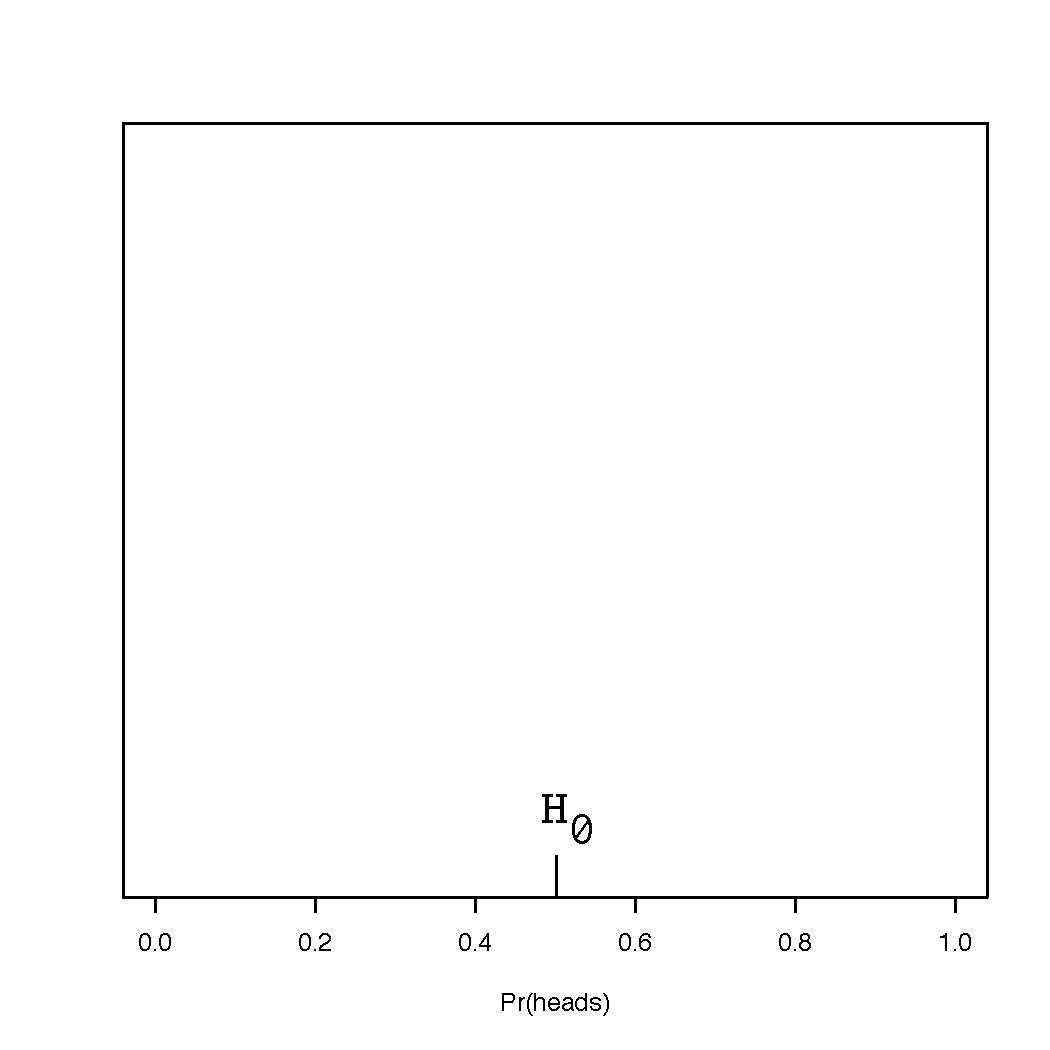
\includegraphics[scale=1.0]{../newimages/coin_axes.pdf}}}
\end{picture}

\myNewSlide
\begin{picture}(500,0)(0,0)
      \put(0,-190){\makebox(0,0)[l]{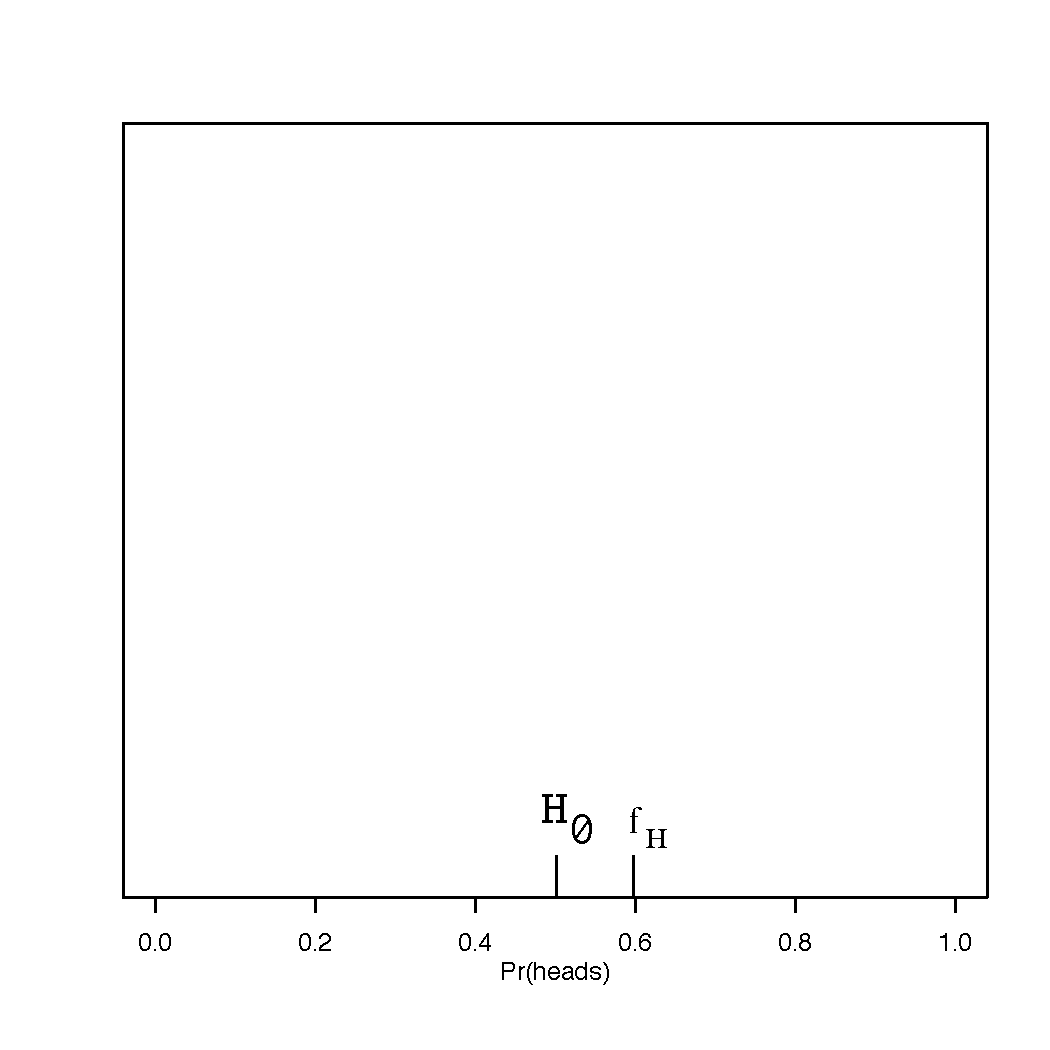
\includegraphics[scale=1.0]{../newimages/coin_axes_data.pdf}}}
\end{picture}

\myNewSlide
\section*{Null distribution}
\begin{picture}(500,0)(0,0)
      \put(0,-190){\makebox(0,0)[l]{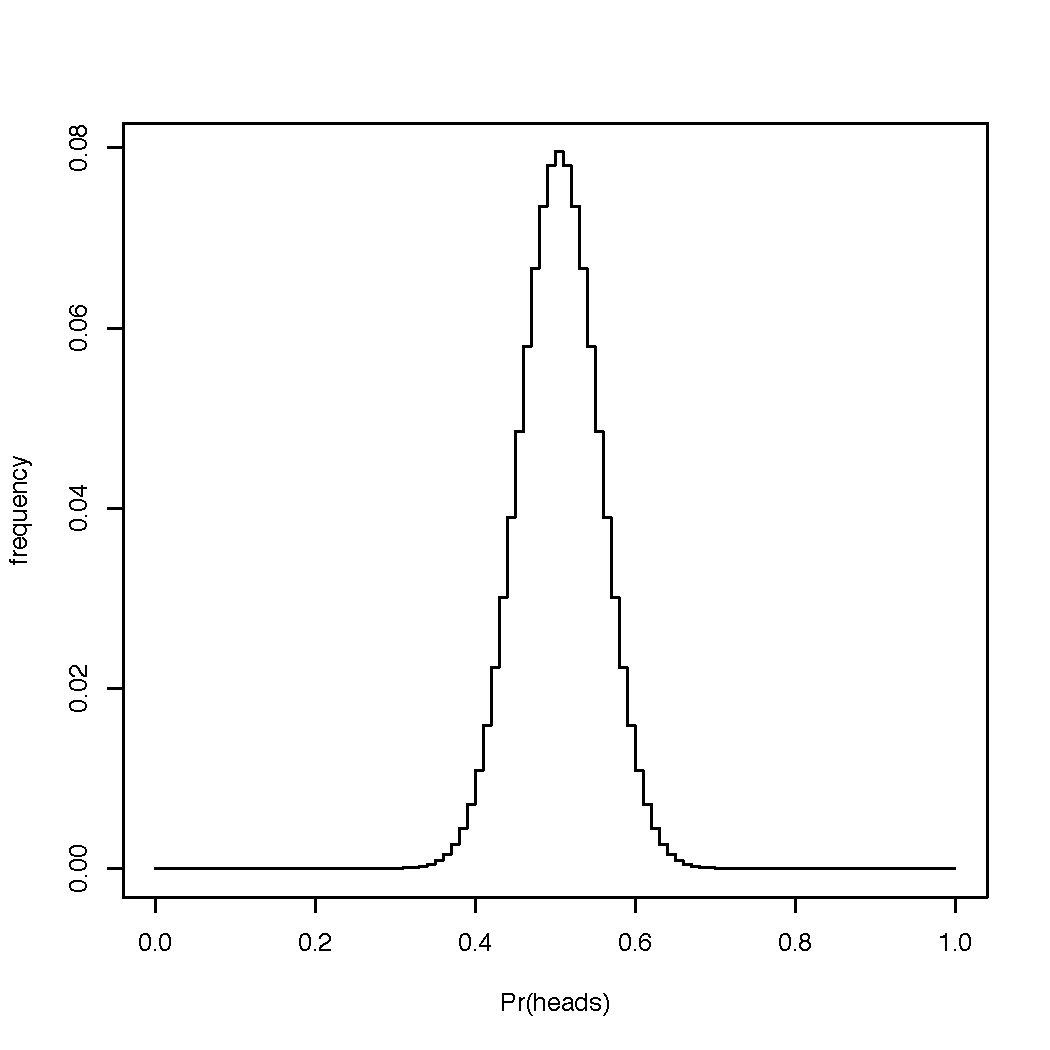
\includegraphics[scale=1.0]{../newimages/coin_wo_tails.pdf}}}
\end{picture}

\myNewSlide
\begin{picture}(500,0)(0,0)
      \put(0,-190){\makebox(0,0)[l]{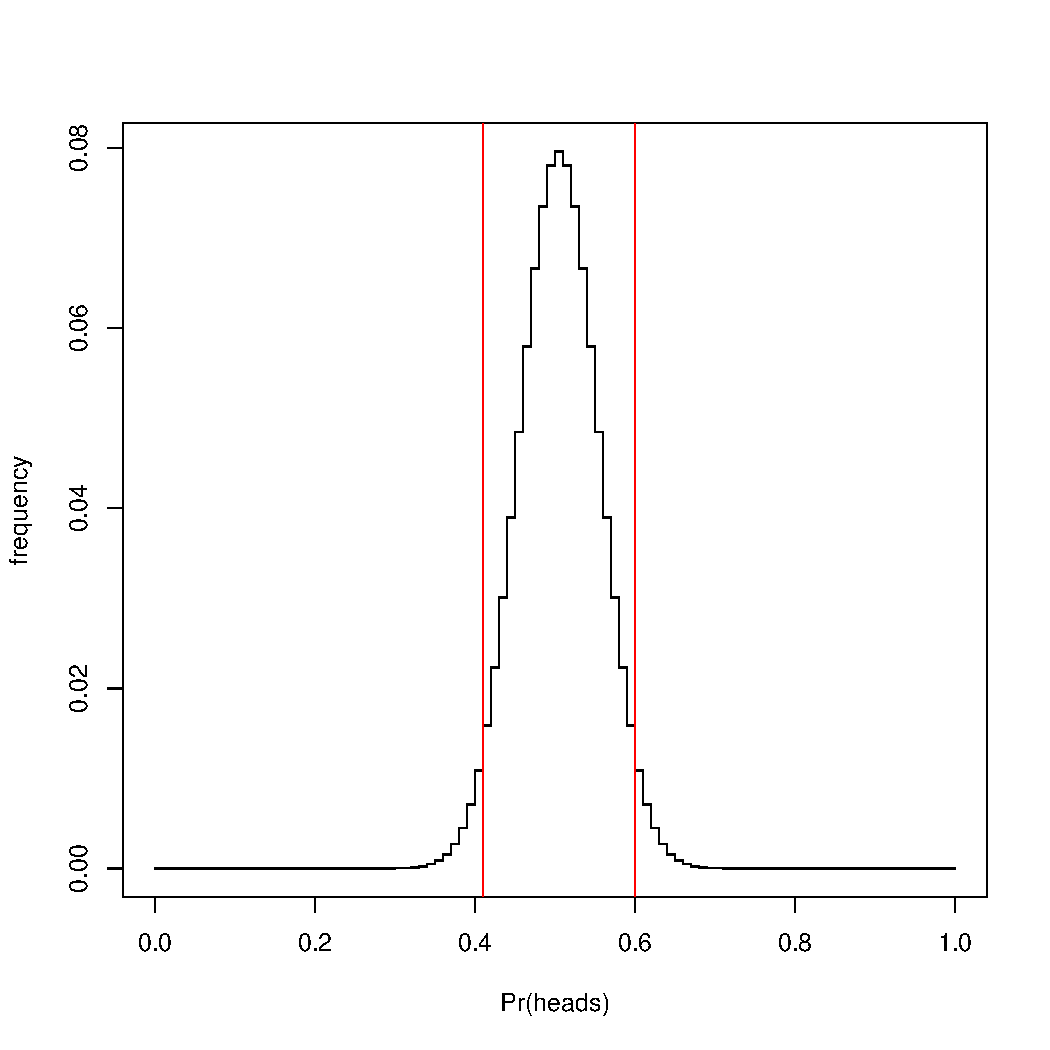
\includegraphics[scale=1.0]{../newimages/coin_w_tails.pdf}}}
      \put(0,-450){$P$-value $\approx$ 0.058}
\end{picture}

\myNewSlide
Making similar plots for tree inference is hard.

\begin{itemize}
    \item Our parameter space is trees and branch lengths.
    \item Our data is a matrix of characters.
    \item It is hard to put these objects on the same. 
    You can do this ``pattern frequency space''. Some projections of this space are:

\end{itemize}




\myNewSlide
\section*{coin flipping}
$N=100$ and $H=60$

Can we reject the hypothesis of a fair coin?

We can use simulation to generate the null distribution (we could actually use the binomial distribution to analytically solve this one)...

\myNewSlide

\begin{picture}(0,0)(0,0)
    \put(-10,-250){\makebox(0,0)[l]{\includegraphics[scale=1.0]{/home/mtholder/Documents/ku_teaching/BIOL-848-2013/images/nullhist.pdf}}}
    \put(150,-250){\color{red} P-value $\approx$ 0.029 }
\end{picture}

\myNewSlide
We discussed how bootstrapping gives us a sense of the variability ofour estimate

It can also give a tail probability for $\Pr(f_H^{(boot)} \leq 0.5)$

Amazingly (for many applications):
$$ \Pr(\hat{f}_H \geq 0.6 \mid \mbox{null is true}) \approx \Pr(f_H^{(boot)} \leq 0.5)$$

In other words, the $P$-value is approximate by the fraction of bootstrap replicates consistent with the null.
\myNewSlide

\begin{picture}(0,0)(0,0)
    \put(-60,-250){\makebox(0,0)[l]{\includegraphics[scale=1.0]{/home/mtholder/Documents/ku_teaching/BIOL-848-2013/images/boothist.pdf}}}
    \put(30,-220){\color{red}$ \Pr(p^{(boot)} \leq 0.5)\approx$ 0.027 }
    \put(30,-265){\color{red}$ BP = \mbox{frac.~of } p^{(boot)} \geq 0.5$}
    \put(30,-310){\color{red}$ BP \approx 0.973$}
    \put(30,-345){\color{red}$ P\mbox{-value} \approx 1-BP$}
\end{picture}

\myNewSlide
\begin{picture}(-0,0)(-0,0)
    \put(60,00){\makebox(30,-150)[l]{\includegraphics[scale=0.5]{/home/mtholder/Documents/ku_teaching/BIOL-848-2013/images/nullhist.pdf}}}
    \put(60,-260){\makebox(30,-150)[l]{\includegraphics[scale=0.5]{/home/mtholder/Documents/ku_teaching/BIOL-848-2013/images/boothist.pdf}}}
\end{picture}







\myNewSlide
\begin{itemize}
    \item When you decide between trees, the boundaries between tree hypotheses can be curved 
    \item When the boundary of the hypothesis space is curved, 1 - BP can be a poor approximation of the $P$-value. -- \citet{EfronHH1996}
\end{itemize}

\myNewSlide
\begin{picture}(-0,0)(-0,0)
    \put(-10,-90){\makebox(30,-150)[l]{\includegraphics[scale=1.2]{../newimages/straight_p_value.pdf}}}
    \put(300,-90){\makebox(30,-150)[l]{\includegraphics[scale=1.2]{../newimages/straight_boot_p_value.pdf}}}
    \put(40,0){\large In the straight border case, symmetry implies that:}
    \put(-20,-150){\large The actual $P$-value (blue region)}
    \put(420,-150){\large $\approx 1-BP$}
    \put(420,-190){\large ($1-BP$ is the blue below)}
\end{picture}

\myNewSlide

\begin{picture}(-0,0)(-0,0)
    \put(-10,-90){\makebox(30,-150)[l]{\includegraphics[scale=1.2]{../newimages/acurved_p_value.pdf}}}
    \put(300,-90){\makebox(30,-150)[l]{\includegraphics[scale=1.2]{../newimages/acurved_boot_p_value.pdf}}}
    \put(40,0){\large In the curved border case, the symmetry breaks down:}
    \put(-20,-150){\large The actual $P$-value (blue region)}
    \put(420,-150){\large $\neq 1-BP$}
    \put(420,-190){\large ($1-BP$ is the blue below)}
\end{picture}

\myNewSlide
\begin{itemize}
    \item \citet{EfronHH1996}  proposed a computationally expensive multi-level bootstrap (which has not been widely used).
    \item \citet{Shimodaira2002} used the same theoretical framework to devise a (more feasible) Approximately Unbiased (AU) test of topologies.
    \begin{itemize}
        \item Multiple scales of bootstrap resampling (80\% of characters, 90\%, 100\%, 110\%$\ldots$) are used to detect and correct for curvature of the boundary.
        \item Implemented in the new versions of PAUP$^{\ast}$
    \end{itemize}
\end{itemize}

\myNewSlide
\section*{\cite{Susko2010} adjusted BP -- aBP}
\large
\begin{compactitem}
    \item Susko agrees with curvature arguments of \citet{EfronHH1996} and \citet{Shimodaira2002}, {\bf but} points out that they ignore the {\bf sharp point} in parameter space around the polytomy.

    \item He correct bootstrap proportions:  $1-aBP$ accurately estimates the $P$-value.

    \item The method uses the multivariate normal distributions the based on calculations about the curvature of the {\em likelihood} surface.

    \item You need to perform a different correction when you know the candidate tree {\em a priori} versus when you are putting BP on the ML tree.

    \item BP may {\bf not} be conservative when you correct for selection bias.
\end{compactitem}

\myNewSlide
\begin{picture}(-0,0)(-0,0)
    \put(-60,-150){\makebox(30,-150)[l]{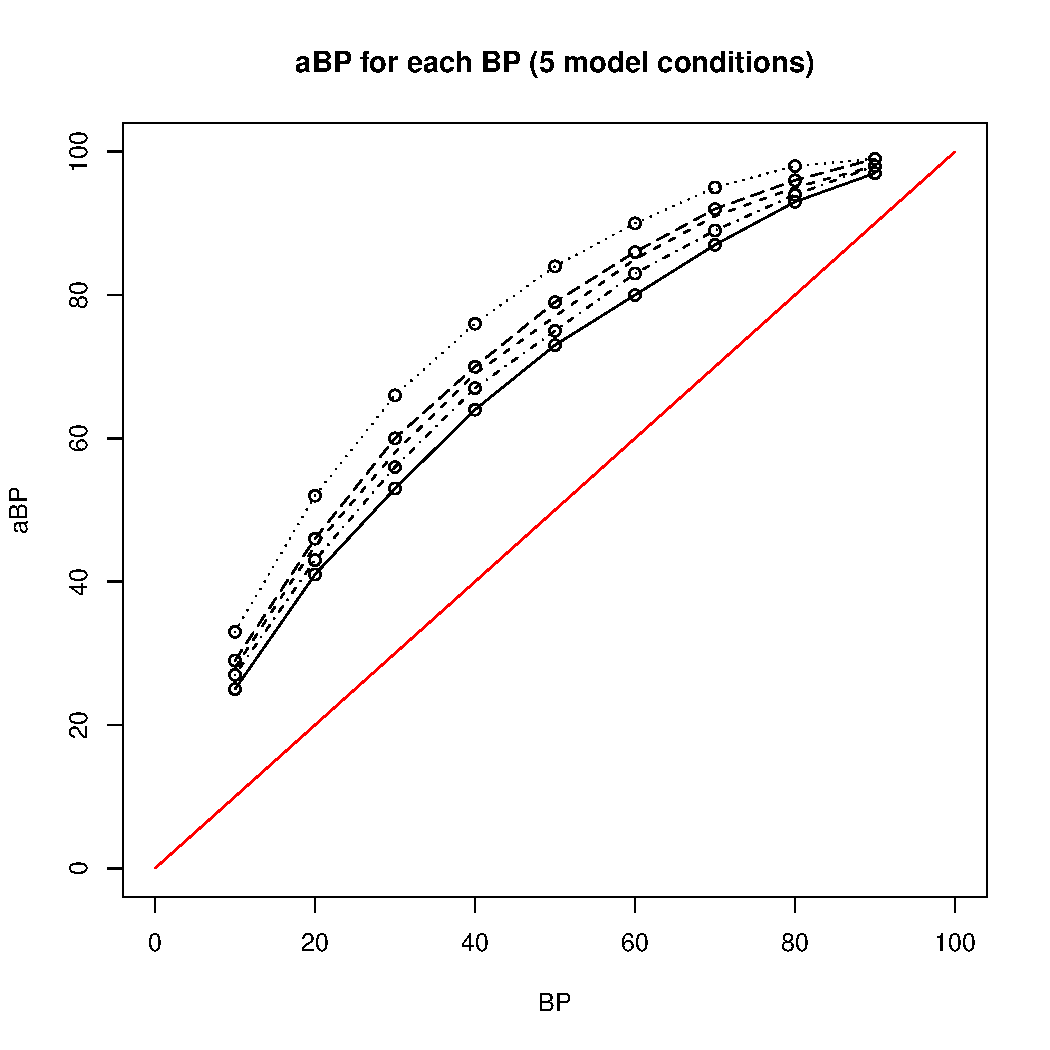
\includegraphics[scale=0.75]{../scripts/Susko2010Table3aBP.pdf}}}
    \put(300,-150){\makebox(30,-150)[l]{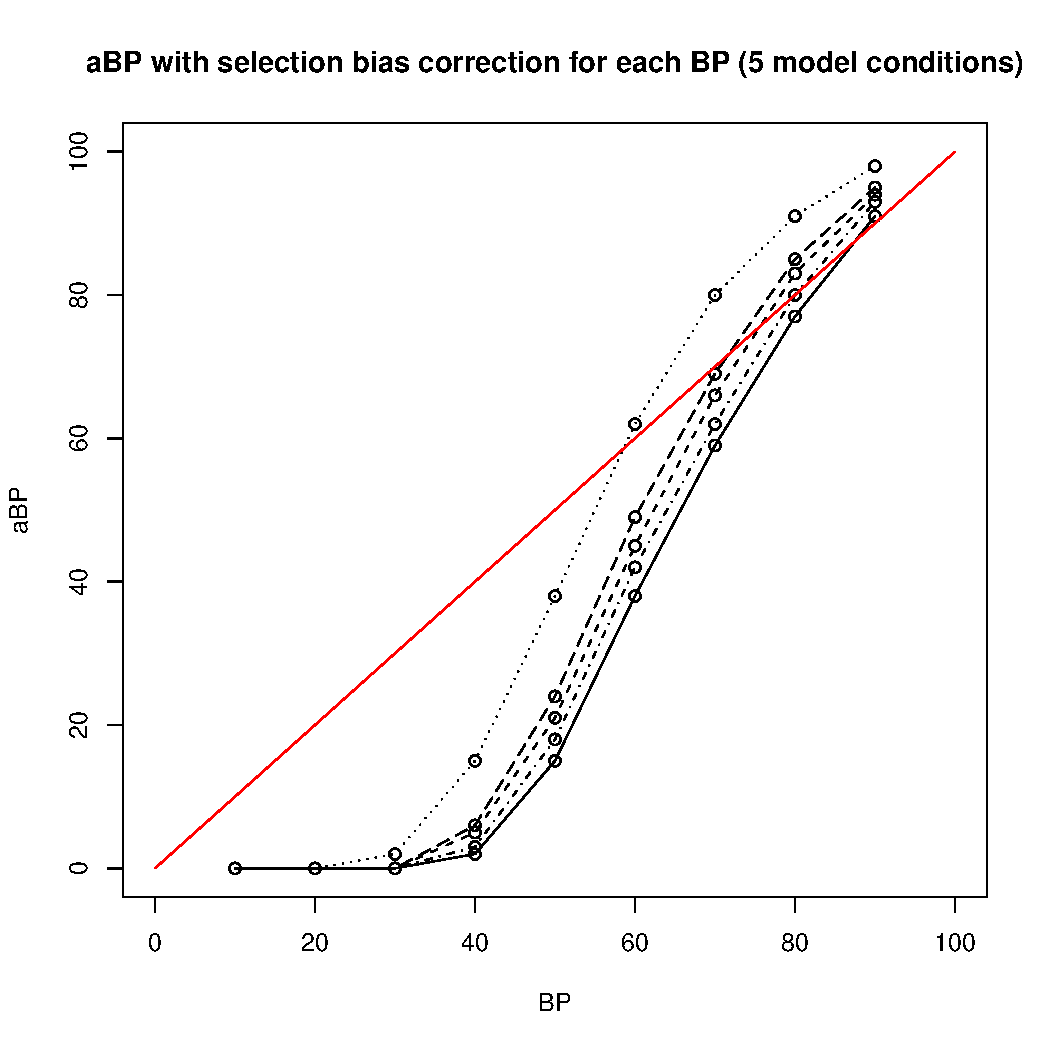
\includegraphics[scale=0.75]{../scripts/Susko2010Table3aBPMLCorrection.pdf}}}
\end{picture}

\myNewSlide
\section*{Conclusions -- bootstrapping}\large
\large
\begin{compactenum}
    \item Non-parametric bootstrapping proportions help us see which branches
    have so little support that they could be plausibly explained by sampling error.
    \item BPs are a little hard to interpret  precisely.
    \item Susko has and adjustment (``aBP``) so that $1 - aBP\approx P$-value for the hypothesis that a recovered branch is not present in the true tree. 
\end{compactitem}


%

\myNewSlide
\large
\begin{picture}(500,0)(0,0)
      \put(-200,-190){\makebox(0,0)[l]{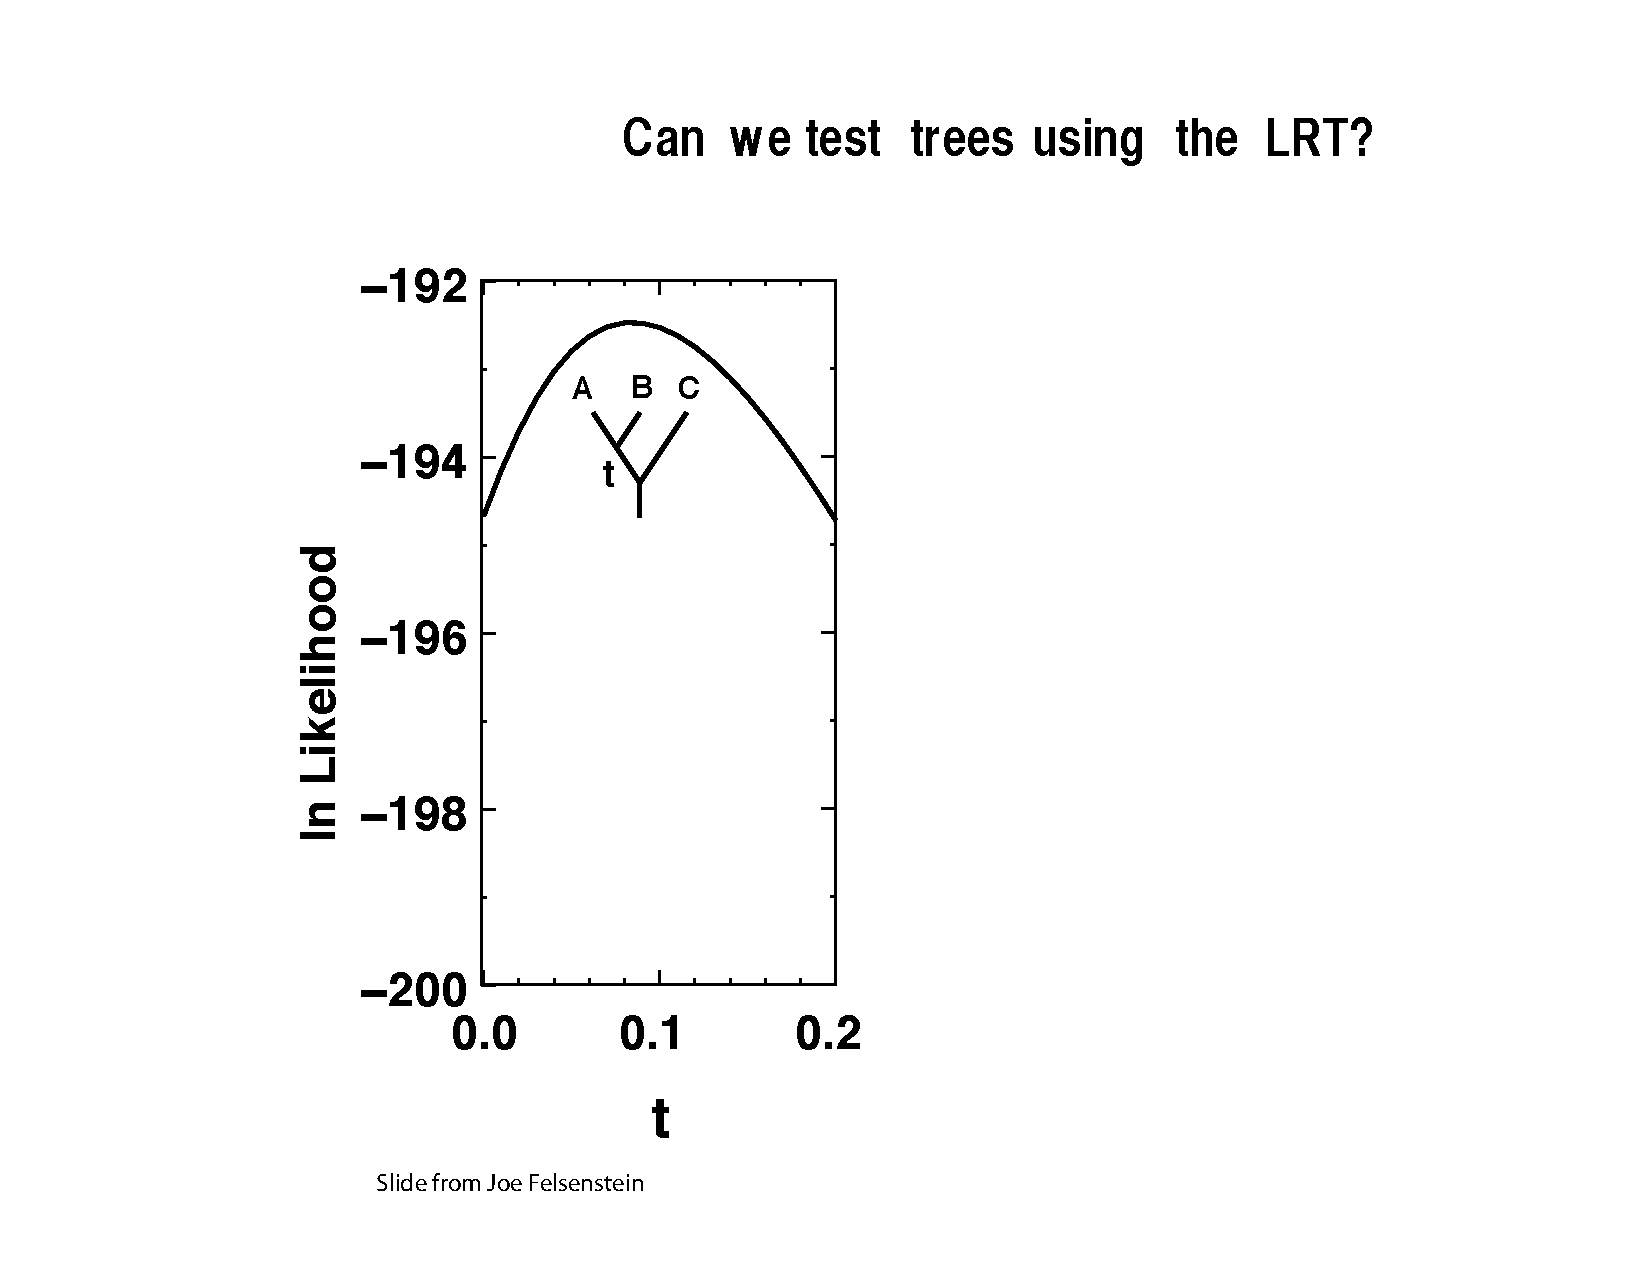
\includegraphics[scale=1.0]{../newimages/JoeFelsTreeLRT1.pdf}}}
      \put(250,-100){1. Should we calculate the LRT as:}
      \put(224,-140){$\delta_i = 2\left[\ln L(t=\hat{t},T_i \mid X) - \ln L(t=0,T_i \mid X)\right]$}
      \put(250,-250){2. And can we use the $\chi_1^2$ distribution to}
      \put(250,-290){get the critical value for $\delta$?}
\end{picture}

\myNewSlide
\begin{picture}(500,0)(0,0)
      \put(-200,-190){\makebox(0,0)[l]{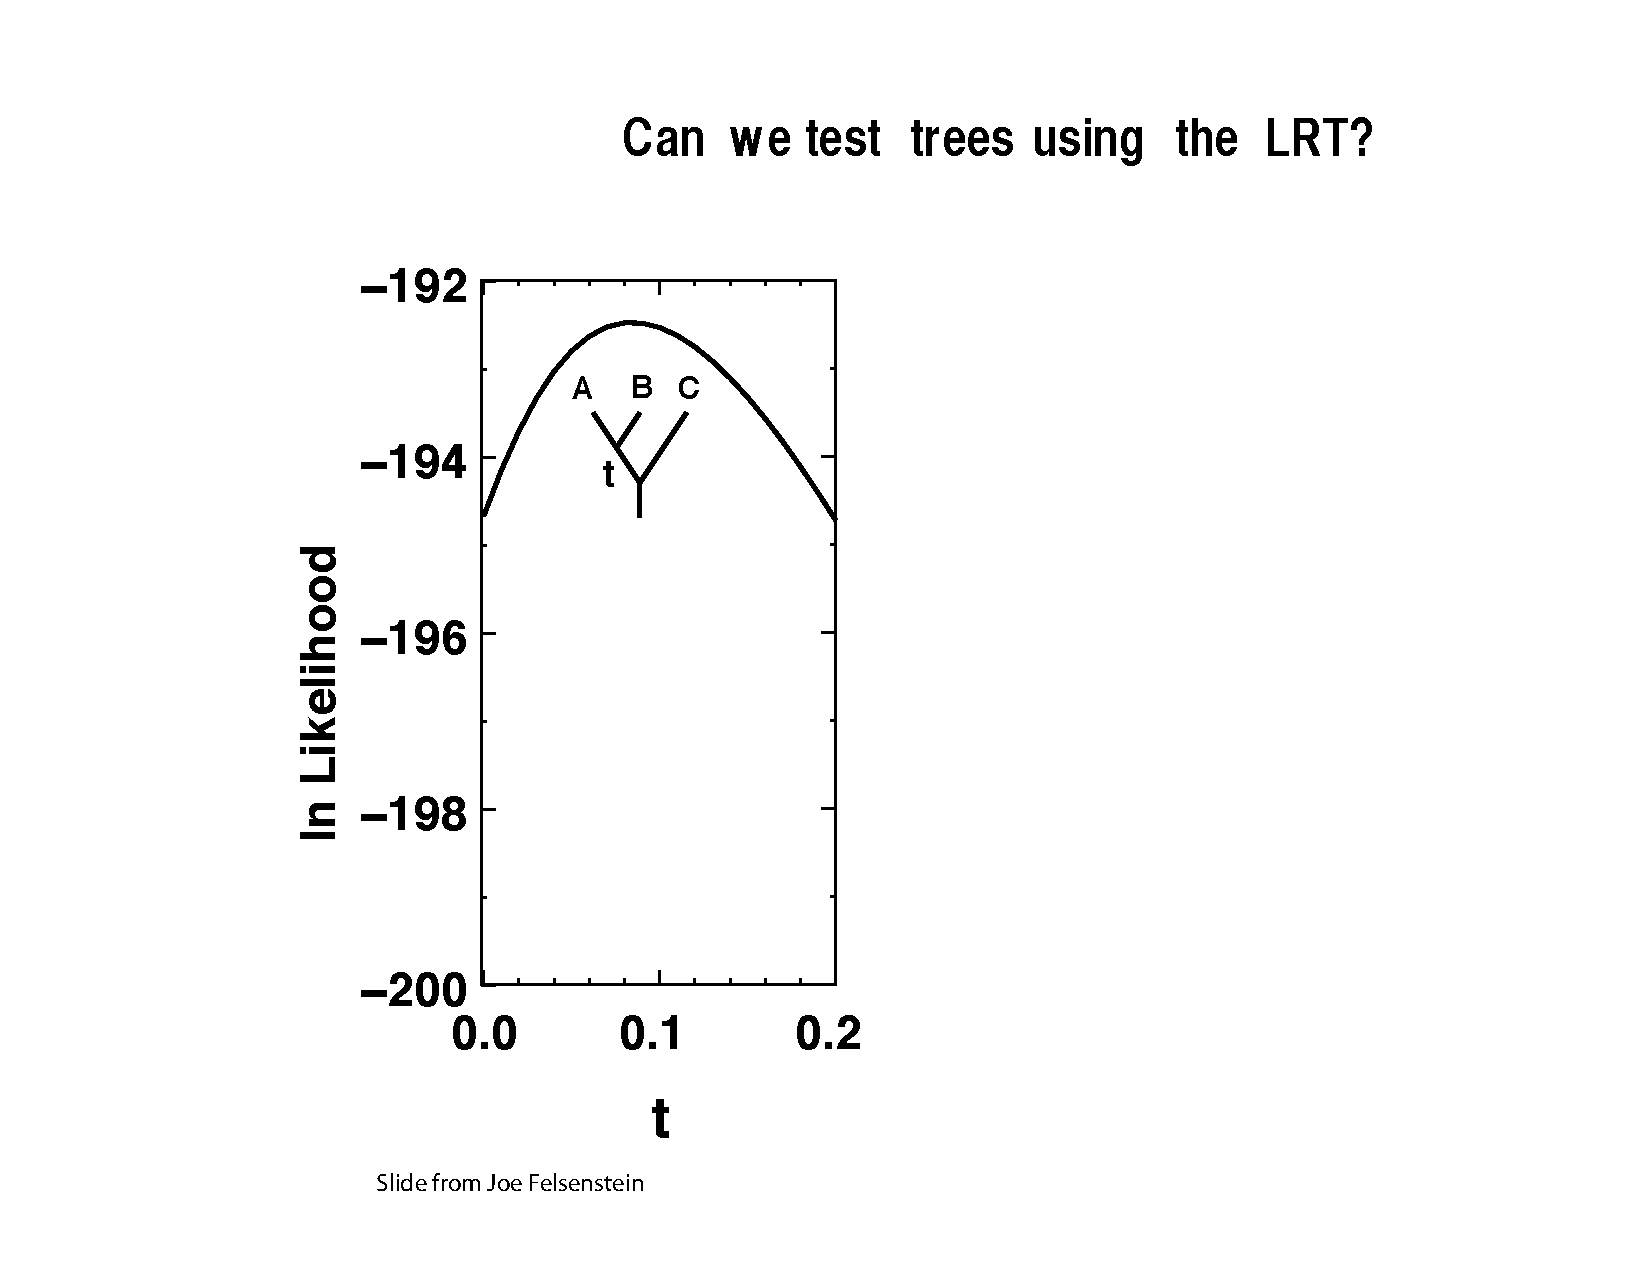
\includegraphics[scale=1.0]{../newimages/JoeFelsTreeLRT1.pdf}}}
      \put(250,-100){1. Should we calculate the LRT as:}
      \put(224,-140){$\delta_i = 2\left[\ln L(t=\hat{t},T_i \mid X) - \ln L(t=0,T_i \mid X)\right]$}
      \put(250,-180){{\bf \color{red}No. $t=0$ might not yield the best}}
      \put(260,-220){\bf\color{red} alternative $\ln L$}
      \put(250,-290){2. And can we use the $\chi_1^2$ distribution to}
      \put(250,-330){get the critical value for $\delta$ ?}
      \put(250,-370){{\bf \color{red}No. Constraining parameters}}
      \put(260,-410){{\bf \color{red}at boundaries leads to a mixture}}
      \put(260,-450){{\bf \color{red}such as: $\frac{1}{2}\chi_0^2 + \frac{1}{2}\chi_1^2$}}
      \put(260,-490){\small See \citet{OtaWHSK2000}.}
\end{picture}


\myNewSlide
\begin{picture}(500,0)(0,0)
      \put(-200,-190){\makebox(0,0)[l]{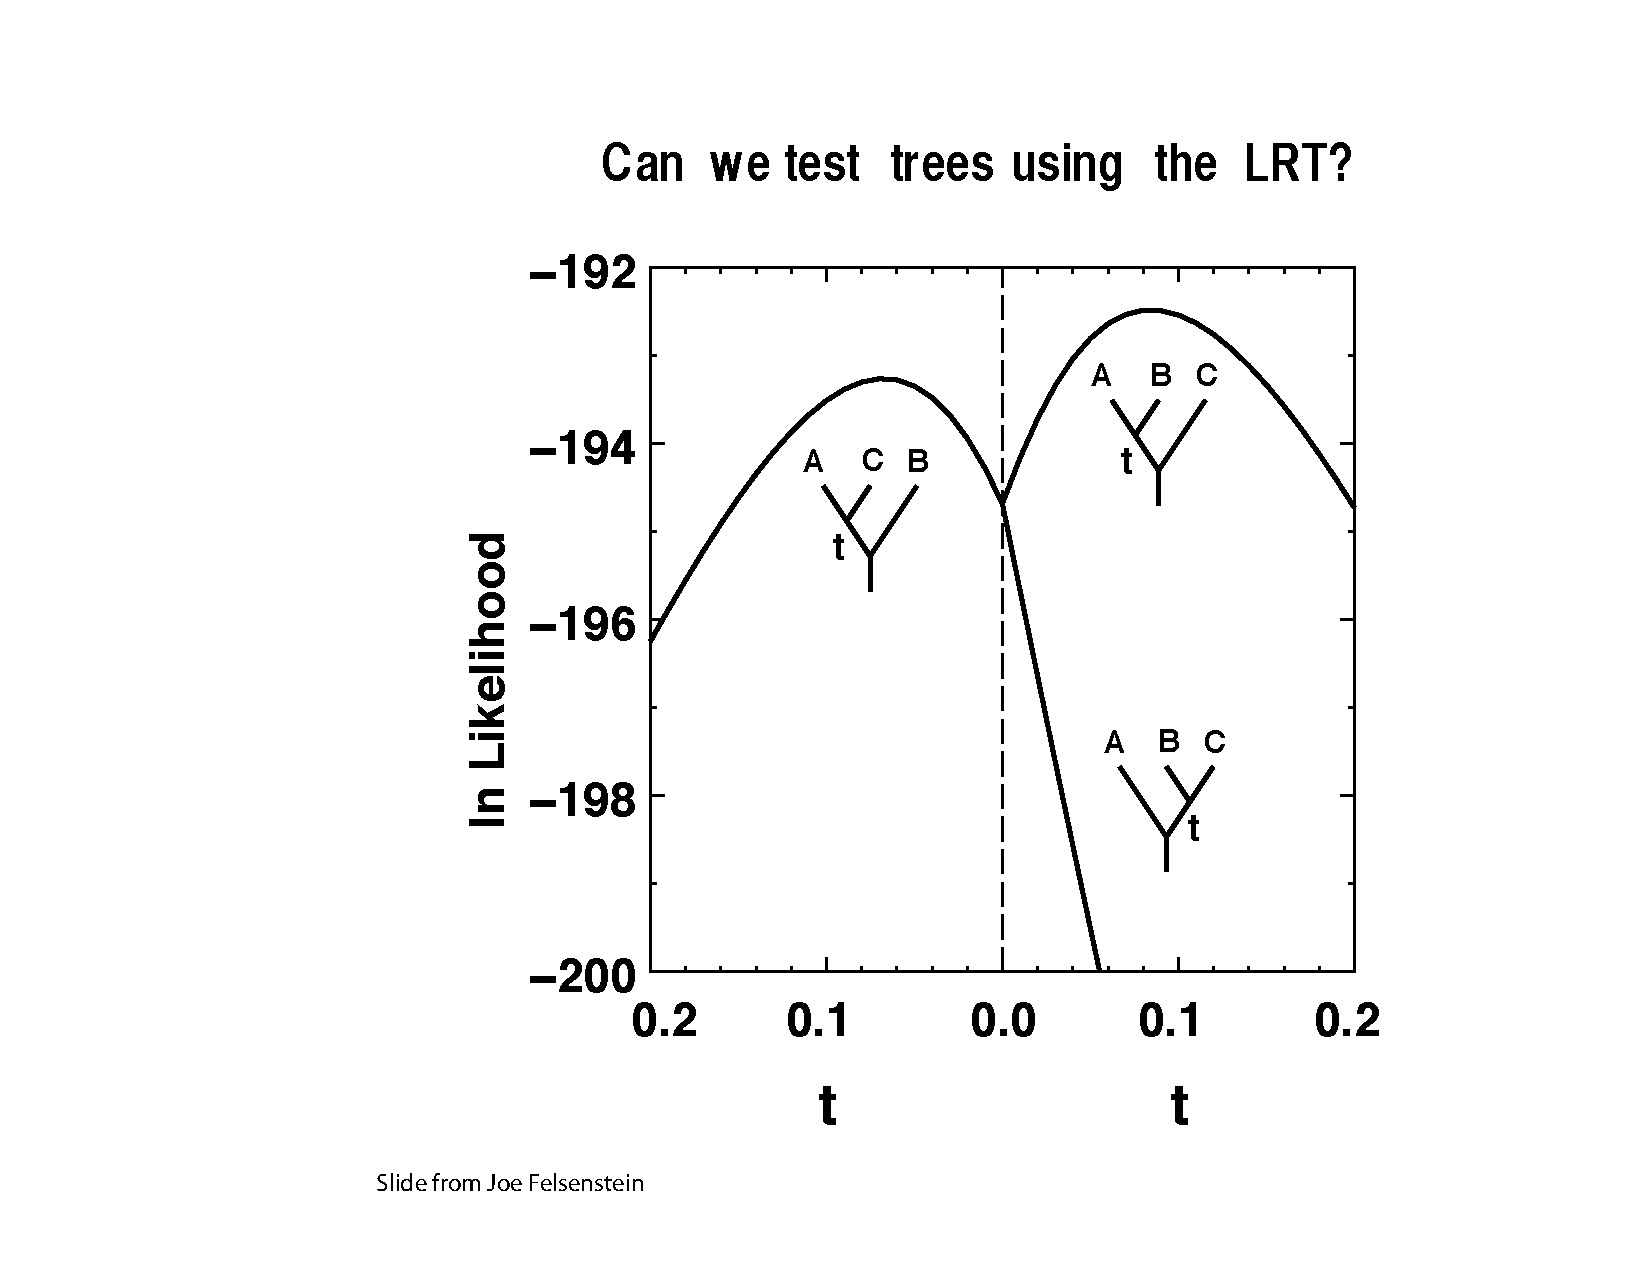
\includegraphics[scale=1.0]{../newimages/JoeFelsTreeLRT2.pdf}}}
      \put(470,-170){{\bf \color{red}No, tree hypotheses}}
      \put(470,-200){{\bf \color{red}are not nested! }}
\end{picture}

\myNewSlide
\section*{aLRT of \citet{AnisimovaG2006}}
\begin{compactitem}
    \item For a {\bf branch} $j$, calculate $\delta_{j}^{\dag}$ as twice the difference in $\ln L$ between the optimal tree (which has the branch) and the best NNI neighbor.
    \item This is very fast.
    \item They argue that the null distribution for each LRT around the polytomy follows a $\frac{1}{2}\chi_0^2 + \frac{1}{2}\chi_1^2$ distribution
    \item The introduce Bonferroni-correction appropriate for correcting for the selection of the best of the three resolutions.
    \item They find aLRT to be accurate and powerful in simulations, but \citet{AnisimovaGDDG2011} report that it rejects too often and is sensitive to model violation.
\end{compactitem}

\myNewSlide
\begin{picture}(500,0)(0,0)
      \put(-130,-450){\makebox(0,0)[l]{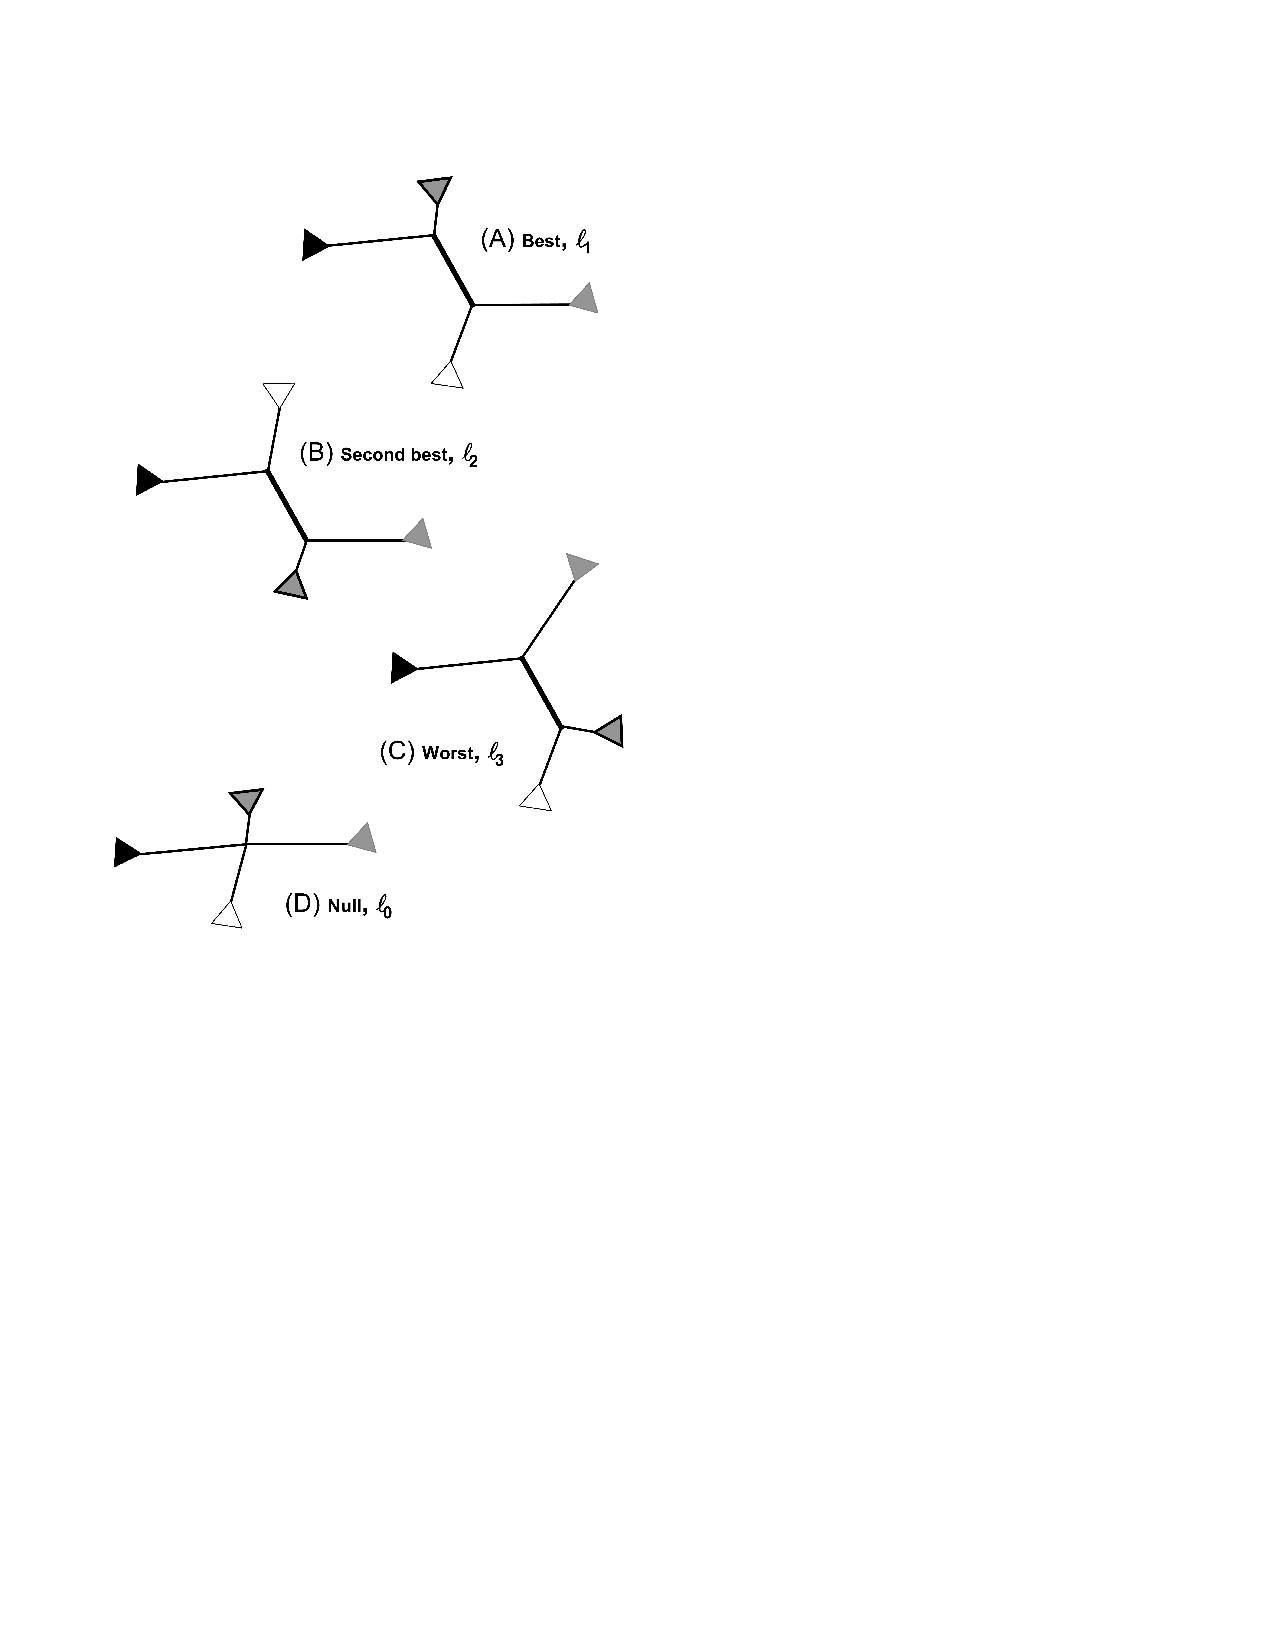
\includegraphics[scale=1.5]{../newimages/AnisimovaG2006Fig1.pdf}}}
      \put(300,-200){aLRT = $2\left[\ln \ell_1 - \ln L(T_2 \mid X)\right]$}
      \put(300,-240){$\ell_1 = L(T_1 \mid X)$}
      \put(400,-400){\small Image from \citet{AnisimovaG2006}}
\end{picture}

\myNewSlide
\section*{aBayes \citet{AnisimovaGDDG2011} }


$$\mbox{aBayes}(T_1 \mid X) = \frac{\Pr(X \mid T_1)}{\Pr(X \mid T_1) + \Pr(X \mid T_2) + \Pr(X \mid T_3)}$$

Simulation studies of \citet{AnisimovaGDDG2011} show it to have the best power of the methods that do not have inflated probability of falsely rejecting the null.

It is sensitive to model violation.

This is similar to ``likelihood-mapping'' of \citet{StrimmerVH1997}


\myNewSlide
\section*{coin flipping example (again, for inspiration)}
$N=100$ and $H=60$

Can we reject the hypothesis of a fair coin?

We can use simulation to generate the null distribution (we could actually use the binomial distribution to analytically solve this one)...


\myNewSlide
\begin{picture}(0,0)(0,0)
    \put(-10,-250){\makebox(0,0)[l]{\includegraphics[scale=1.0]{/home/mtholder/Documents/ku_teaching/BIOL-848-2013/images/nullhist.pdf}}}
    \put(150,-250){\color{red} P-value $\approx$ 0.029 }
\end{picture}

\myNewSlide
\section*{The simplest phylogenetic test would compare two trees}
\Large
Null: If we had no sampling error (infinite data) $T_1$ and $T_2$ would explain the data equally well. 

Test Statistic: $$\delta(T_1,T_2 \mid X) = 2\left[\ln L(T_1 \mid X) - \ln L(T_2 \mid X)\right]$$

Expectation under null: $$\mathbb{E}_{H_0}\left[\delta(T_1,T_2 \mid X)\right] = 0$$


\myNewSlide
\begin{picture}(500,0)(-20,-50)
      \put(20,-20){\small Using 3000 sites of mtDNA sequence for 5 primates}
      \put(20,-60){\normalsize $T_1$ is ((chimp, gorilla), human)}
      \put(50,-200){\makebox(0,-190)[l]{\includegraphics[scale=1.0]{../scripts/mtdna/chimpGorilla3000sites.pdf}}}
\end{picture}



\includepdf{/home/mtholder/Documents/storage/talks/teaching/WoodsHole/treeTesting2016/take5/hcg-score-table-txt-diff-by-site.pdf}

\includepdf{/home/mtholder/Documents/storage/talks/teaching/WoodsHole/treeTesting2016/take5/hcg-score-table-txt-scatterplot.pdf}

\myNewSlide
\begin{picture}(500,0)(-20,-50)
      \put(20,-20){\small Using 3000 sites of mtDNA sequence for 5 primates}
      \put(20,-60){\normalsize $T_1$ is ((chimp, gorilla), human)   \hskip2cm $\ln L(T_1 \mid X) = -7363.296$}
      \put(20,-100){\normalsize $T_2$ is ((chimp, human), gorilla)  \hskip2cm $\ln L(T_2 \mid X) = -7361.707$}
      \put(-10,-385){\small$\delta(T_1,T_2 \mid X)=-3.18$}
      \put(300,-385){\small$\mathbb{E}(\delta)$}
      \put(50,-150){\makebox(0,-190)[l]{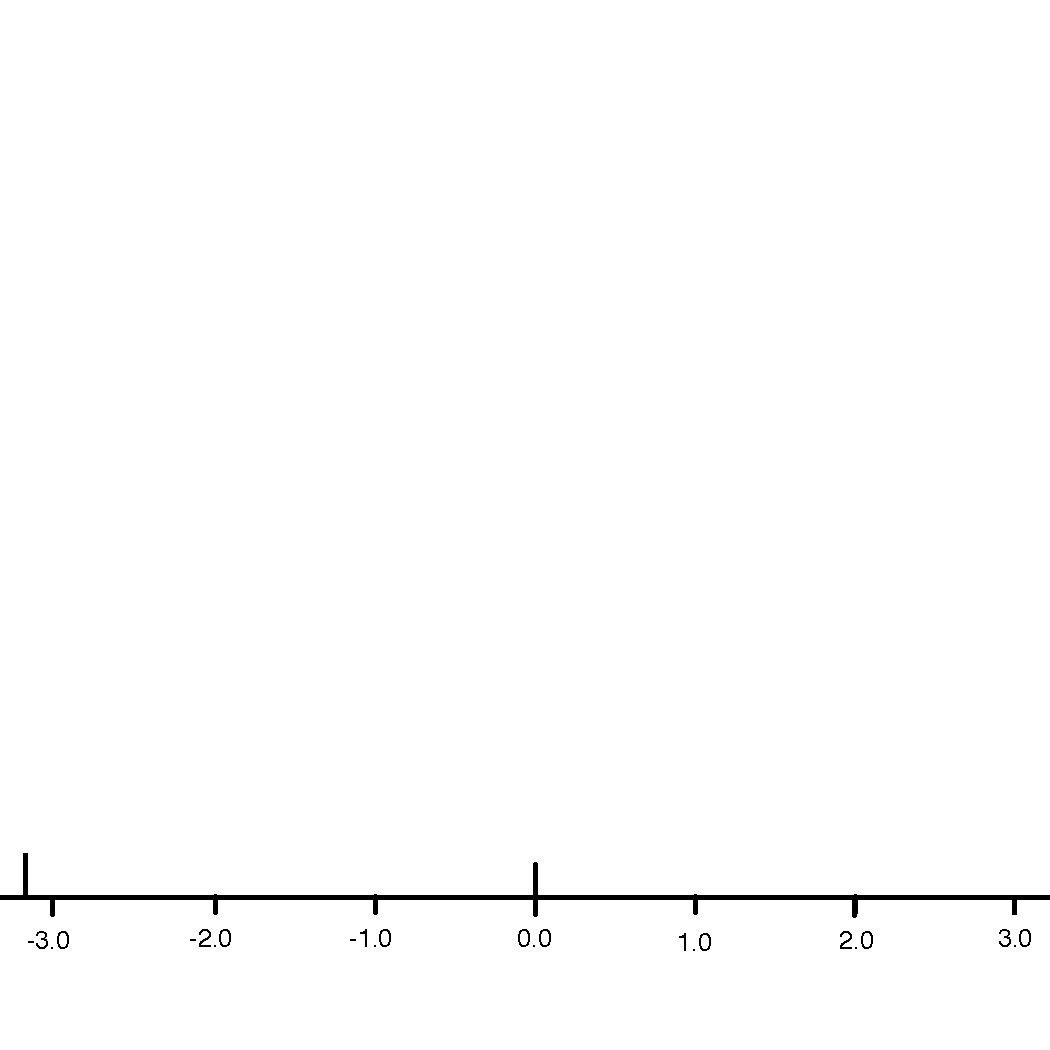
\includegraphics[scale=1.0]{../newimages/delta_axes.pdf}}}
      \put(220,-480){$\delta(T_1,T_2 \mid X) $}
\end{picture}




\myNewSlide

To get the $P$-value, we need to know the probability: $$\Pr\left(\big | \delta(T_1,T_2 \mid X)\big |  \geq 3.18  {\bm{\Big|}}  H_0\mbox{ is true}\right) $$
\begin{picture}(500,0)(-20,-50)
      \put(-10,-235){\small$\delta(T_1,T_2 \mid X)=-3.18$}
      \put(460,-235){\small$-\delta(T_1,T_2 \mid X)=3.18$}
      \put(10,-270){\huge$\leftarrow$}
      \put(570,-270){\huge$\rightarrow$}
      \put(300,-235){\small$\mathbb{E}(\delta)$}
      \put(50,-0){\makebox(0,-190)[l]{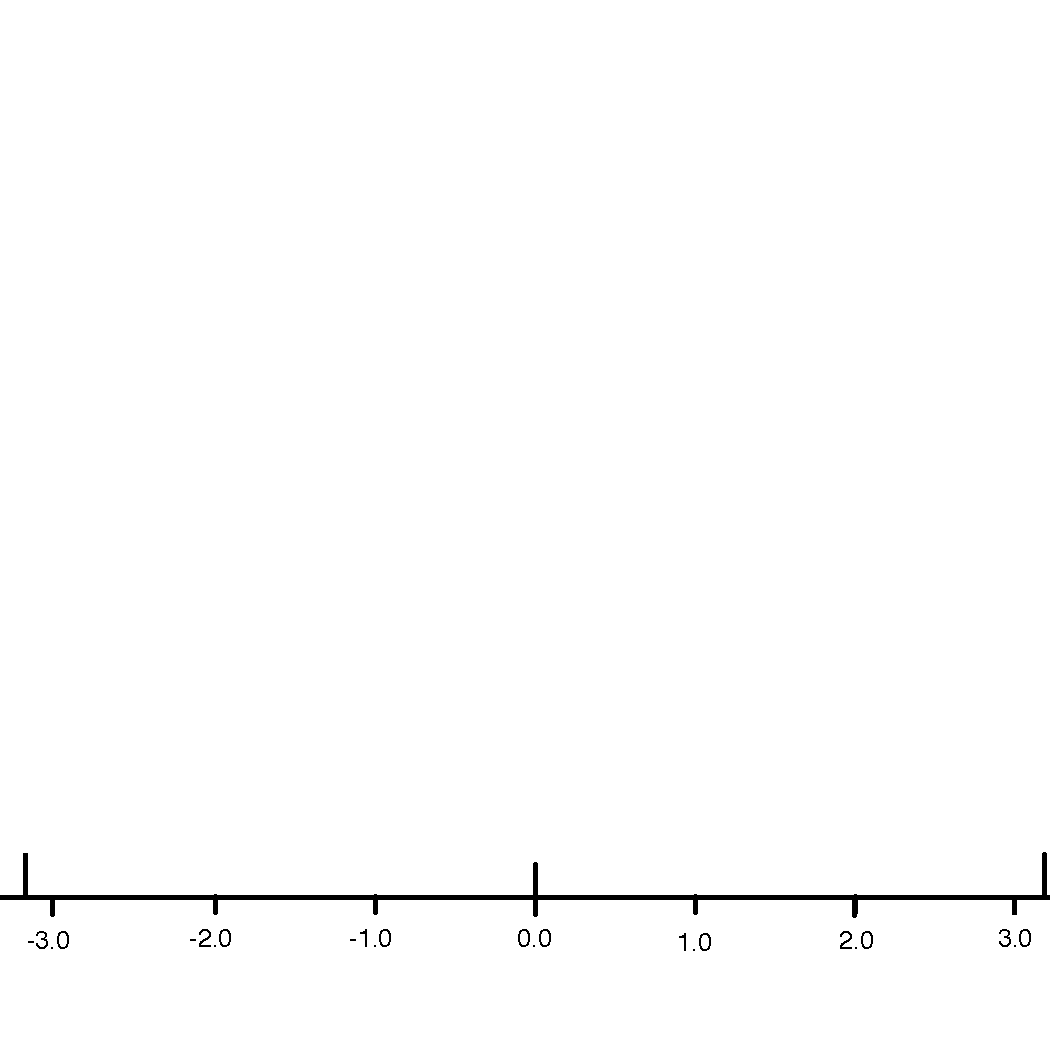
\includegraphics[scale=1.0]{../newimages/delta_axes_reflected.pdf}}}
      \put(220,-330){$\delta(T_1,T_2 \mid X) $}
\end{picture}

\myNewSlide
\section*{KH Test}
\begin{compactenum}
    \item Examine the difference in $\ln L$ for each site: $\delta(T_1,T_2 \mid X_i)$ for site $i$.
    \item Note that the total difference is simply a sum:
        $$\delta(T_1,T_2 \mid X) = \sum_{i=1}^M\delta(T_1,T_2 \mid X_i)$$
    \item The variance of $\delta(T_1,T_2 \mid X)$ will be a function of the variance in ``site'' $\delta(T_1,T_2 \mid X_i)$ values.
\end{compactenum}



\myNewSlide
\begin{picture}(500,0)(0,0)
      \put(0,10){\large $\delta(T_1,T_2 \mid X_i)$ for each site, $i$.}
      \put(280,-35){\large $\vdots$}
      \put(20,-250){\makebox(0,0)[l]{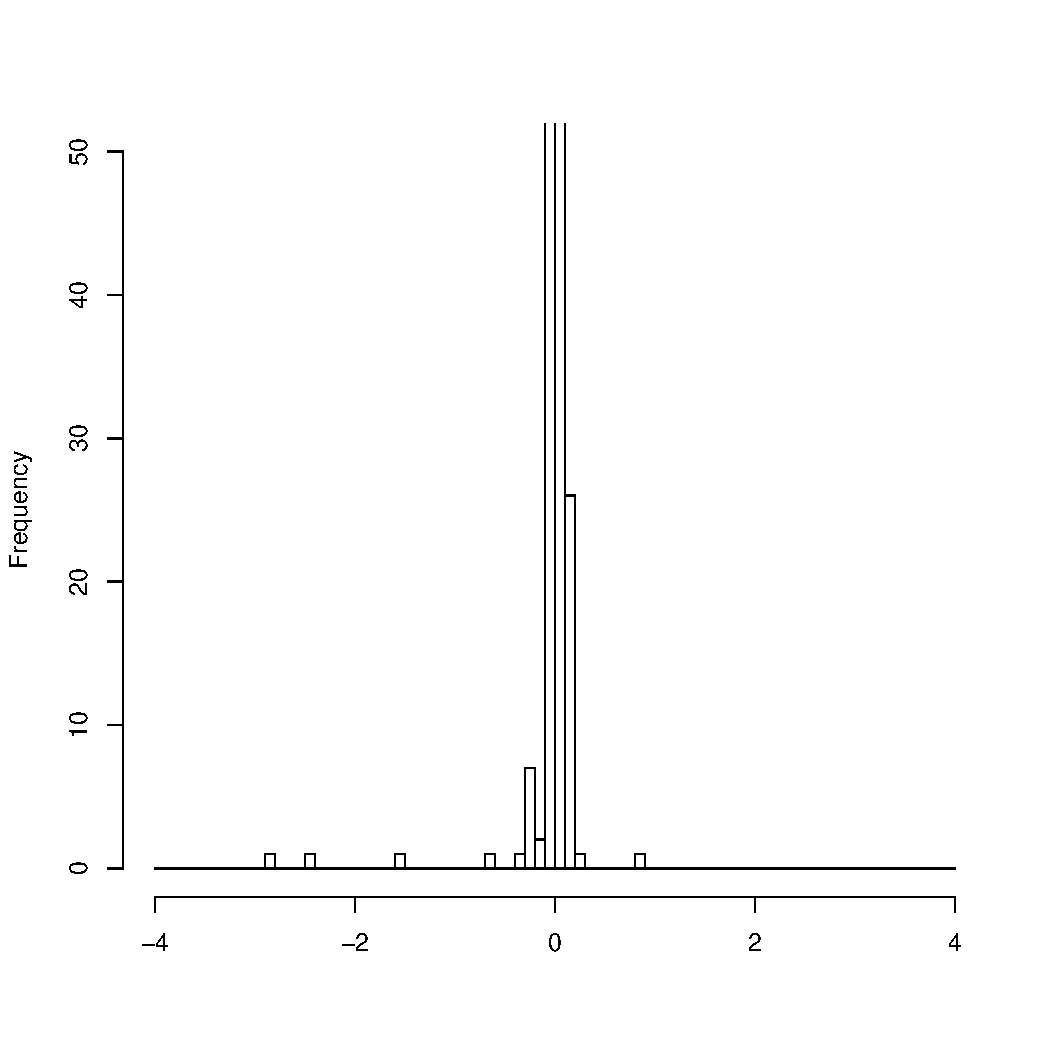
\includegraphics[scale=1.0]{../scripts/mtdna/d1-2hist.pdf}}}
      \put(250,-490){\normalsize$\delta(T_1,T_2 \mid x_i)$}
\end{picture}


\myNewSlide
\section*{KH Test - the variance of $\delta(T_1,T_2 \mid X)$}
To approximate variance of $\delta(T_1,T_2 \mid X)$ under the null, we could:
\begin{compactenum}
    \item use assumptions of Normality (by appealing to the Central Limit Theorem\footnote{\citet{Susko2014} recently showed that this is flawed and too conservative.}). Or
    \item use bootstrapping to generate a cloud of pseudo-replicate $\delta(T_1,T_2 \mid X^{\ast})$ values, and look at their variance.
\end{compactenum}

\myNewSlide
\begin{picture}(500,0)(0,0)
      \put(0,-10){\large $\delta$ for many (RELL) bootstrapped replicates of the data}
      \put(20,-250){\makebox(0,0)[l]{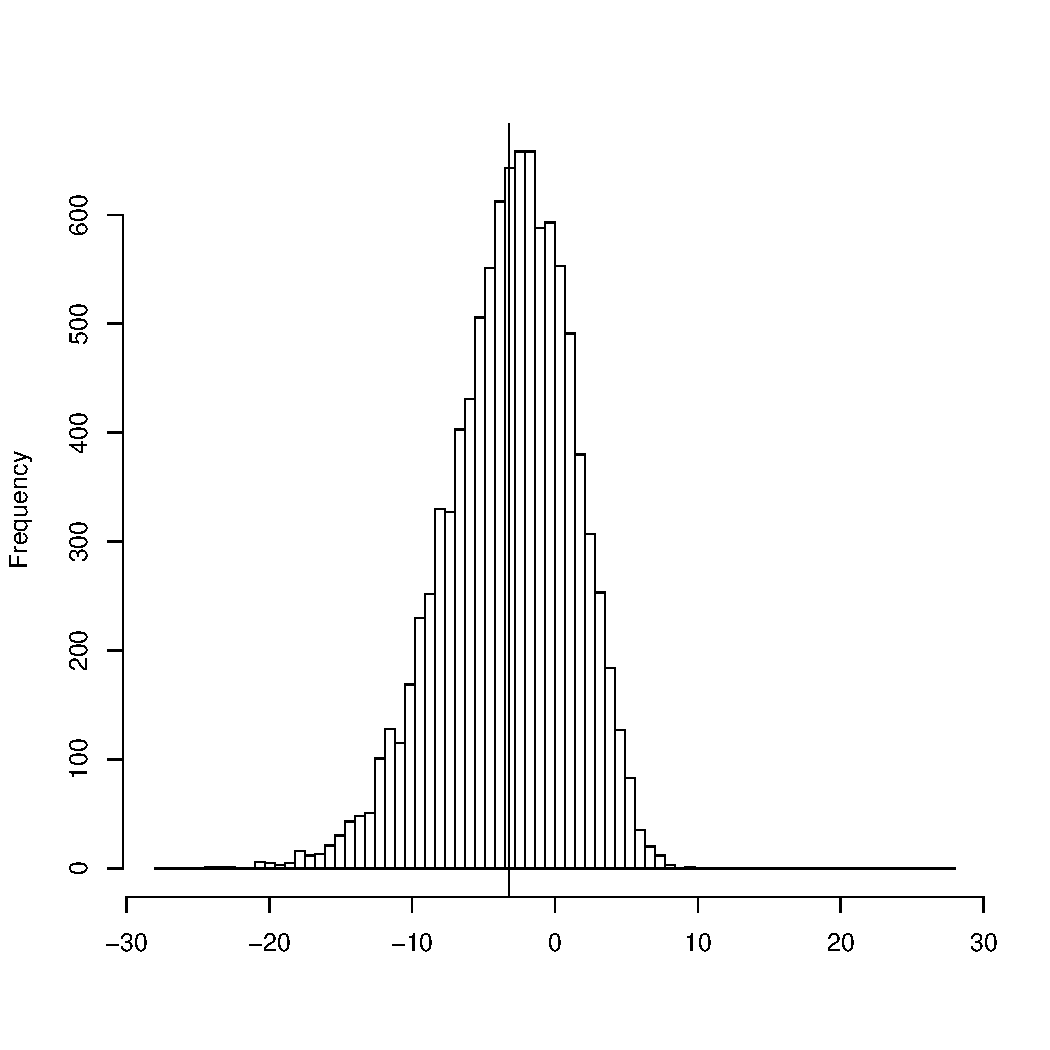
\includegraphics[scale=1.0]{../scripts/mtdna/uncentered1-2hist.pdf}}}
      \put(250,-490){\normalsize$\delta(T_1,T_2 \mid X^{\ast})$}
\end{picture}



\myNewSlide
\begin{picture}(500,0)(0,0)
      \put(0,10){\large The (RELL) bootstrapped sample of statistics.}
      \put(0,-20){\large Is this the null distribution for our $\delta$ test statistic?}
      \put(20,-250){\makebox(0,0)[l]{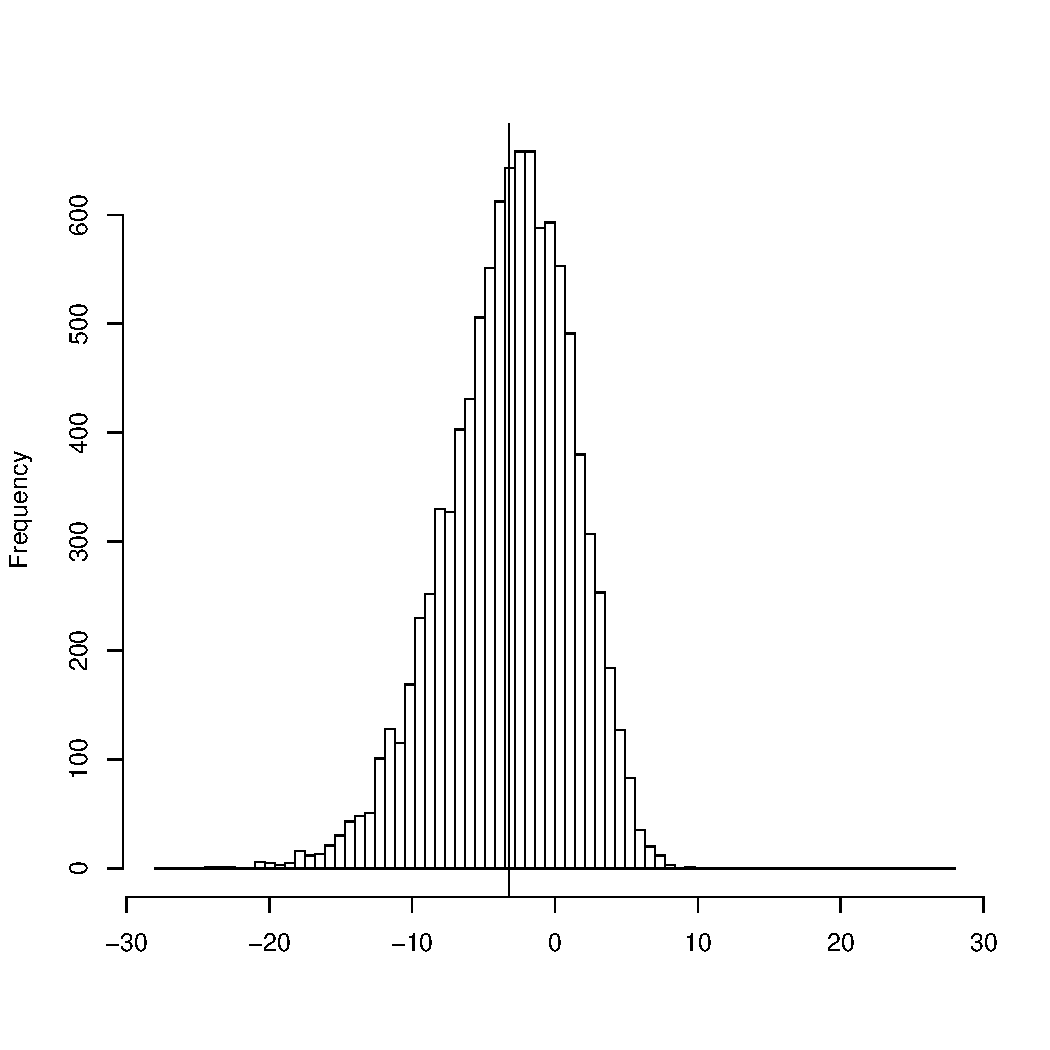
\includegraphics[scale=1.0]{../scripts/mtdna/uncentered1-2hist.pdf}}}
      \put(250,-490){\normalsize$\delta(T_1,T_2 \mid X^{\ast})$}
\end{picture}

\myNewSlide
\section*{KH Test - `centering'}
{\begin{center} $\mathbb{E}_{H_0}\left[\delta(T_1,T_2 \mid X)\right] = 0$\end{center}}
Bootstrapping gives us a reasonable guess of the variance under $H_0$

Subtracting the mean of the bootstrapped $\delta(T_1,T_2 \mid X^{\ast})$ values gives the null distribution.

For each of the $j$ bootstrap replicates, we treat $$\delta(T_1,T_2 \mid X^{\ast j}) - \bar\delta(T_1,T_2 \mid X^{\ast})$$  as draws from the null distribution.

\myNewSlide
\begin{picture}(500,0)(0,0)
      \put(0,10){\large $\delta(T_1,T_2 \mid X^{(j)})-\bar\delta(T_1,T_2 \mid X^{\ast})$}
      \put(0,-25){for many (RELL) bootstrapped replicates of the data}
      \put(20,-250){\makebox(0,0)[l]{\includegraphics[scale=1.0]{../scripts/mtdna/centered1-2hist.pdf}}}
      \put(150,-490){\normalsize$\delta(T_1,T_2 \mid X^{(j)})-\bar\delta(T_1,T_2 \mid X^{\ast})$}
\end{picture}

\myNewSlide
\begin{picture}(500,0)(0,0)
      \put(0,10){Approximate null distribution with}
      \put(0,-30){tails (absolute value $\geq 3.18$) shown}
      \put(20,-250){\makebox(0,0)[l]{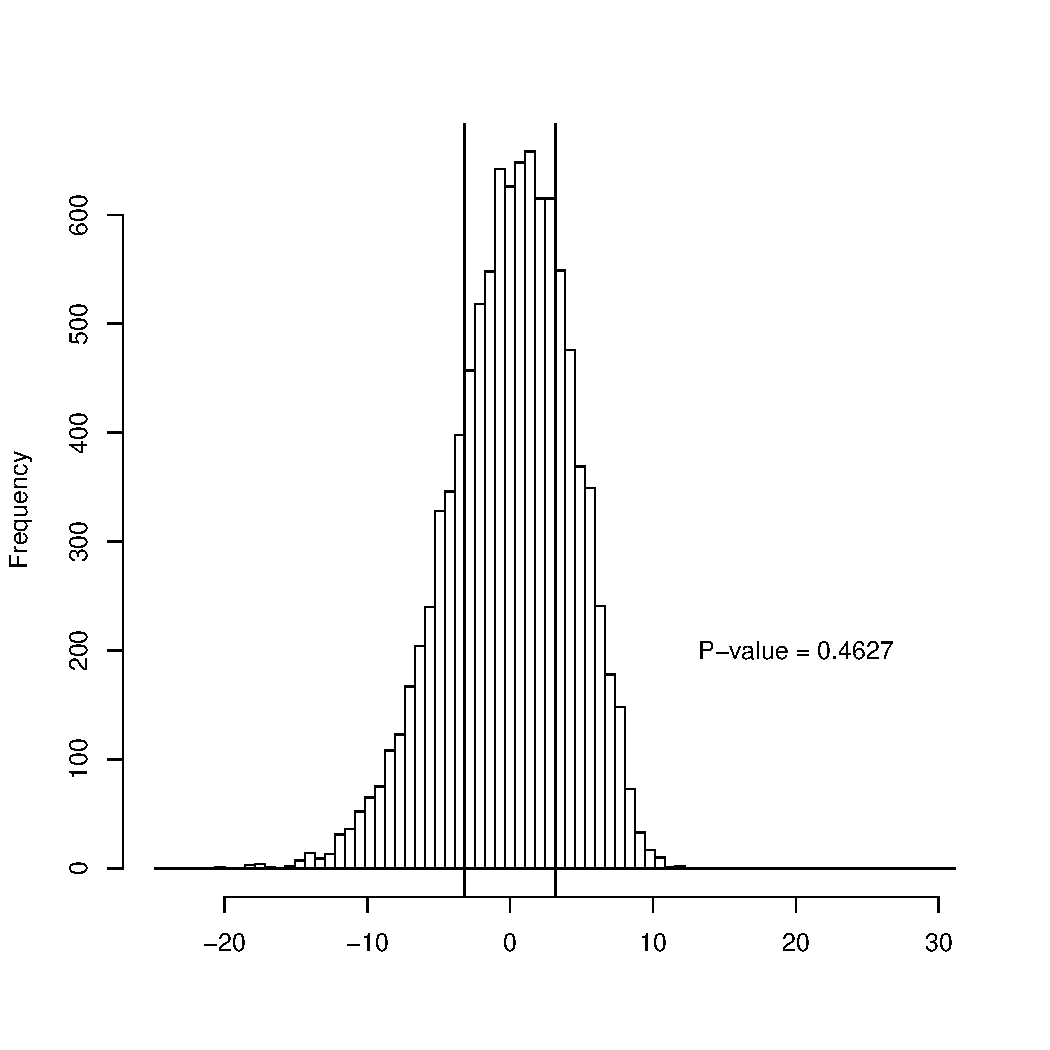
\includegraphics[scale=1.0]{../scripts/mtdna/centered1-2hist-p.pdf}}}
      \put(175,-490){\normalsize$\delta(T_1,T_2 \mid X^{\ast})-\bar\delta(T_1,T_2 \mid X^{\ast})$}
\end{picture}




\myNewSlide
\section*{Other ways to assess the null distribution of the LR test statistic}
\begin{itemize}
    \item Bootstrapping then centering LR, and 
    \item Using normality assumptions.
\end{itemize}
are both clever and cute solutions.

They are too conservative \citep{Susko2014} - more complicated calculations from the Normal [KHns] or mixtures of $\chi^2$ distributions [chi-bar].

They do not match the null distribution under any model of sequence evolution.


\myNewSlide
\section*{Mini-summary}

\begin{itemize}
    \item $\delta(T_1,T_2 \mid X) = 2\left[\ln L(T_1 \mid X) - \ln L(T_2 \mid X)\right]$ is a powerful statistic for discrimination between trees.
    \item We can assess confidence by considering the variance in signal between different characters.
    \item Bootstrapping helps us assess the variance in $\ln L$ that we would expect to result from sampling error.
\end{itemize}



%\myNewSlide
\section*{Scenario}\normalsize
\begin{enumerate}
    \item A (presumably evil) competing lab scoops you by publishing a tree, $T_1$, for your favorite group of organisms.
    \item You have just collected a new dataset for the group, and your ML estimate of the best tree, $T_2$, differ's from $T_1$.
    \item A KH Test shows that your data {\bf significantly} prefer $T_2$ over $T_1$.
    \item You write a (presumably scathing) response article.
\end{enumerate}
Should a {\em Systematic Biology} publish your response?

\myNewSlide\large
\section*{What if start out with only one hypothesized tree, and we want to compare it to the ML tree?}
The KH Test is {\bf NOT} appropriate in this context \citep[see][for discussion of this point]{GoldmanAR2000}
    
{\bf Multiple Comparisons}: lots of trees increases the variance of $\delta(\hat{T},T_1 \mid X)$\\

{\bf Selection bias}: Picking the ML tree to serve as one of the hypotheses invalidates the centering procedure of the KH test.

\myNewSlide
\section*{Using the ML tree in your test introduces selection bias}
Even when the $H_0$ is true, we do not expect $2\left[\ln L(\hat{T}) - \ln L(T_1)\right]= 0$

Imagine a competition in which a large number of equally skilled people compete, and you compare the score of one competitor against the highest scorer.

\myNewSlide
\begin{picture}(500,0)(0,0)
      \put(-10,15){Experiment: 70 people each flip a fair coin 100 times and}
      \put(0,-20){count \# heads.}
      \put(100,-55){$h_1 - h_2$}
      %\put(400,-55){$\max(h) - h_1$}
      \put(-30,-250){\makebox(0,0)[l]{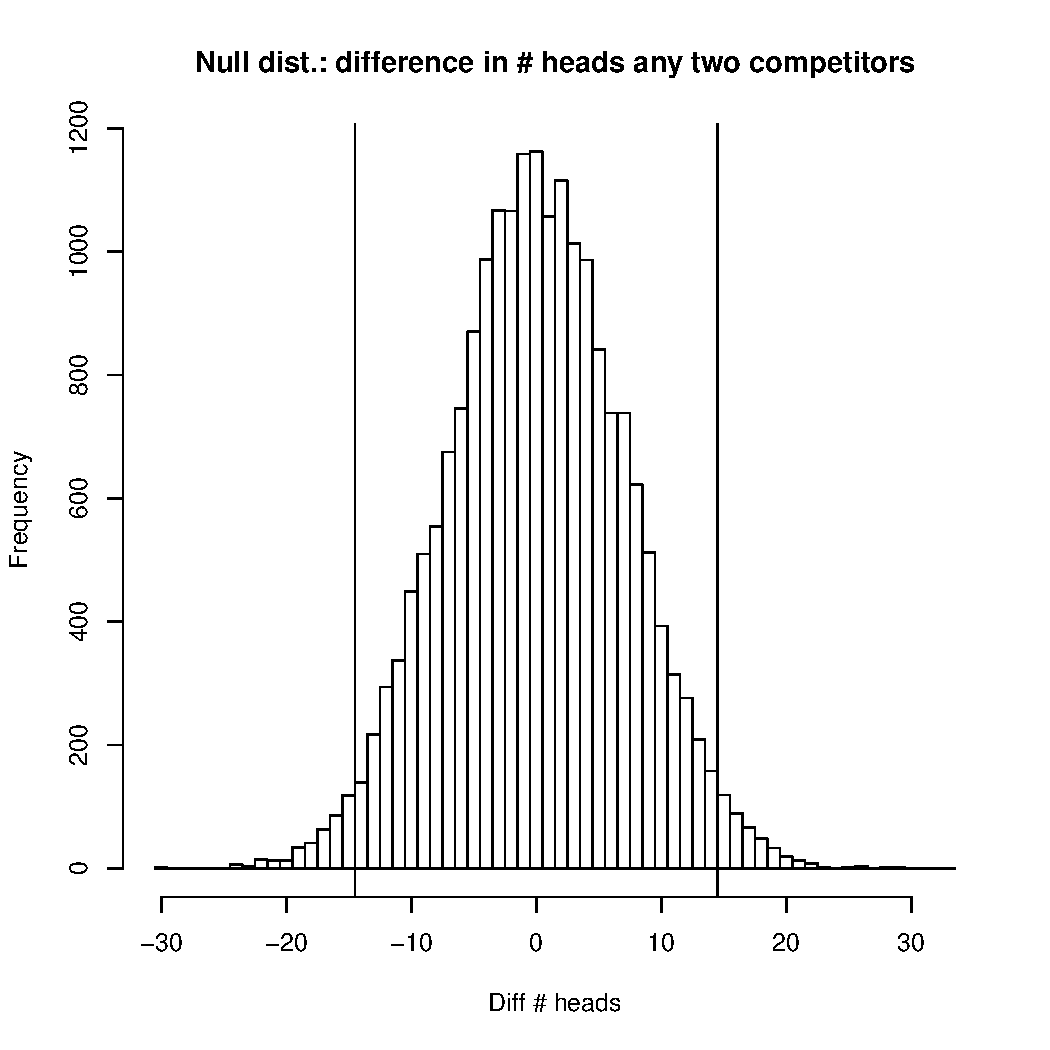
\includegraphics[scale=.75]{../scripts/cfc_diff_a_priori.pdf}}}
\end{picture}

\myNewSlide
\begin{picture}(500,0)(0,0)
      \put(-10,15){Experiment: 70 people each flip a fair coin 100 times and}
      \put(0,-20){count \# heads.}
      \put(100,-55){$h_1 - h_2$}
      \put(400,-55){$\max(h) - h_1$}
      \put(-30,-250){\makebox(0,0)[l]{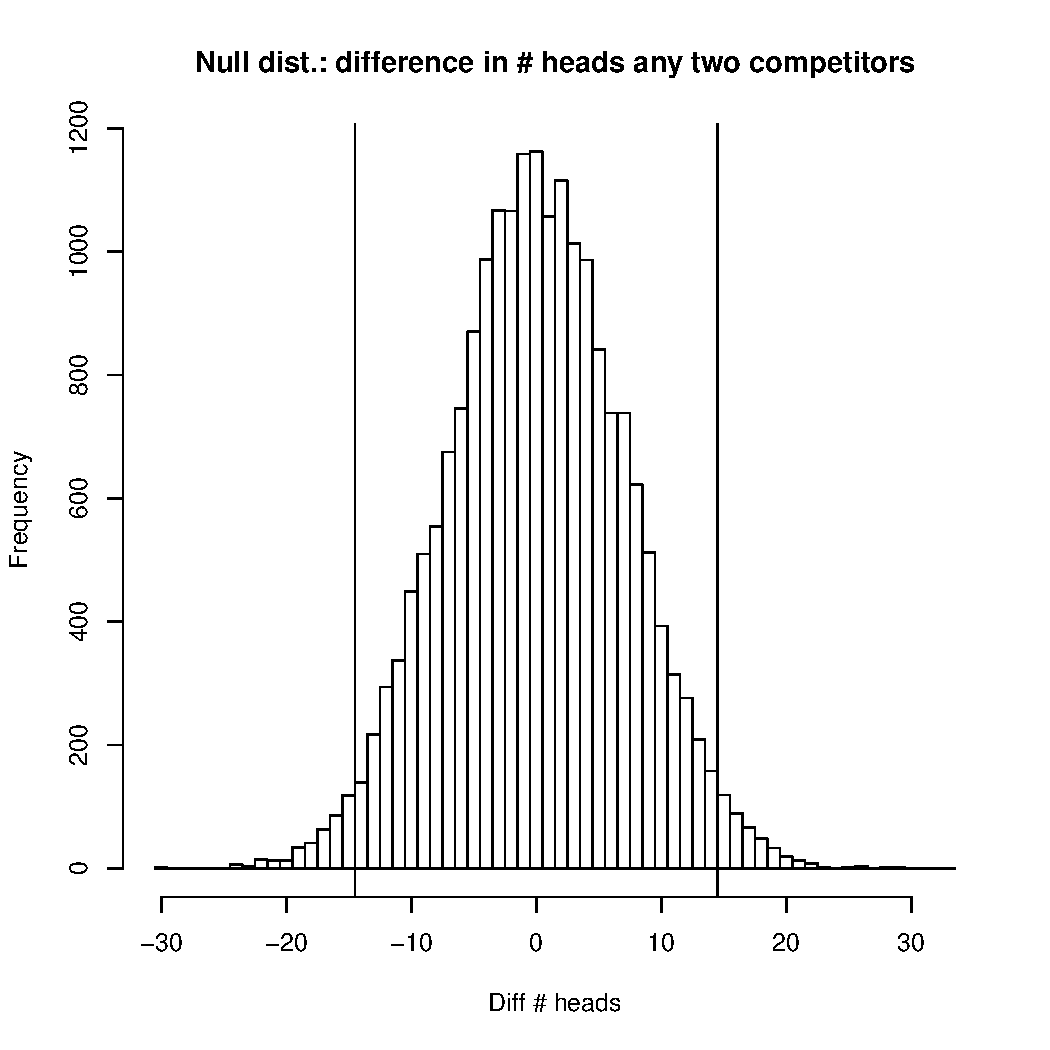
\includegraphics[scale=.75]{../scripts/cfc_diff_a_priori.pdf}}}
      \put(320,-250){\makebox(0,0)[l]{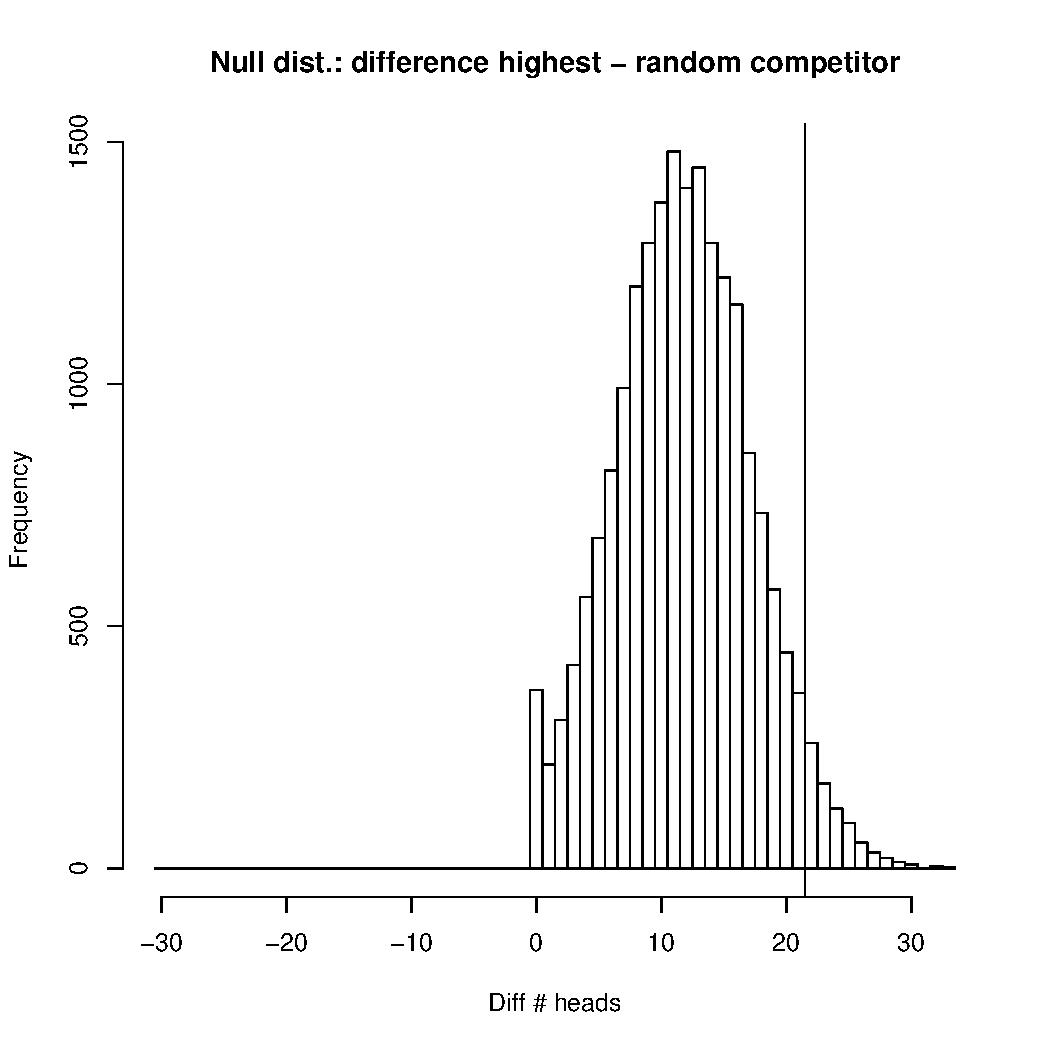
\includegraphics[scale=.75]{../scripts/cfc_diff_best_v_one.pdf}}}
\end{picture}


\myNewSlide 
\section*{Shimodaira and Hasegawa proposed the SH test which deals the ``selection bias'' introduced by using the ML tree in your test}
Requires {\bf set of candidate trees} - these {\bf must not} depend on the dataset to be analyzed.

$H_0$: each tree in the candidate set is as good as the other trees.

The test makes worst-case assumptions - it {\bf is conservative}.

AU test is less conservative (still needs a candidate set)





\myNewSlide
\includepdf[pages={1-4}]{pbootdiagram.pdf} 

\myNewSlide
\section*{Parametric bootstrapping to generate the null distribution for the LR statistic}
\begin{enumerate}
    \item find the best tree and model pair that are consistent with the null,
    \item Simulate many datasets under the parameters of that model,
    \item Calculate $\delta^{(j)} = 2\left[\ln L (\hat{T}^{(j)} \mid  X^{(j)}) - \ln L (\hat{T}_{0}^{(j)} \mid  X^{(j)})\right]$ for each simulated dataset.
        \begin{compactitem}
            \item the $(j)$ is just an index for the simulated dataset,
            \item $\hat{T}_{0}^{(j)}$ is the tree under the null hypothesis for simulation replicate $j$
        \end{compactitem}
\end{enumerate}


\myNewSlide
\section*{Parametric bootstrapping}
This procedure is often referred to as SOWH test (in that form, the null tree is specified {\em a priori}).

\citet{HuelsenbeckHN1996} describes how to use the approach as a test for monophyly.

Intuitive and powerful, but not robust to model violation \citep{Buckley2002}.

Can be done manually\footnote{instructions in \url{https://molevol.mbl.edu/index.php/ParametricBootstrappingLab}}
or via \href{https://github.com/josephryan/sowhat}{SOWHAT} by \citet{SOWHAT}. Optional demo \href{https://molevol.mbl.edu/index.php/SOWHAT}{here}.

\citet{Susko2014}: collapse optimize null tree with 0-length contraints for the branch in question (to avoid rejecting too often)

\myNewSlide
\includepdf[pages={1}]{/home/mtholder/Documents/ku_teaching/BIOL-848-2013/images/gtr_i_g_sim_hist_data.pdf} 


\myNewSlide
\includepdf[pages={1}]{/home/mtholder/Documents/ku_teaching/BIOL-848-2013/images/jc_sim_hist_data.pdf} 

\myNewSlide
\section*{Significantly different genealogy $\neq$ different phylogeny}
\begin{itemize}
    \item True ``gene tree'' can differ from true ``species tree'' for several biological reasons:
    \begin{itemize}
        \item deep coalescence,
        \item gene duplication/loss (you may be comparing paralogs),
        \item lateral gene transfer.
    \end{itemize}
\end{itemize}

%\includepdf[pages={6-18}]{/home/mtholder/Documents/storage/talks/bodega/HolderSotU.pdf} 

\myNewSlide
\section*{We often don't want to test tree topologies}
\begin{itemize}
    \item If we are conducting a ``comparative method'' we have to consider phylogenetic history,
    \item ideally we would integrate out the uncertainty in the phylogeny
\end{itemize}

%\myNewSlide
\section*{Conclusions 1 - confidence on trees}\large
\large
\begin{compactenum}
    \item Non-parametric bootstrapping: useful for assessing sampling error, but a little hard to interpret  precisely.
    \begin{compactitem}
        \item Susko's  aBP gives $1 - aBP\approx P$-value for the hypothesis that a recovered branch is not present in the true tree. 
    \end{compactitem}
    \item ``How should we assign a $P$-value to tree hypothesis?'' is surprisingly complicated.
    \begin{compactitem}
        \item Kishino-Hasegawa (KH-Test) if testing 2 ({\em a priori}) trees.
        \item Shimodaira's approximately unbiased (AU-Test) for sets of trees.
        \item Parametric bootstrapping (can simulate under complex models)
    \end{compactitem}
\end{compactenum}

\myNewSlide
\section*{Conclusions 2 - confidence about evo.~hypotheses}
If $H_0$ is about the evolution of a trait:
\begin{compactenum}
    \item $P$-value must consider uncertainty of the tree:
    \begin{compactitem}
        \item can be large $P$ over confidence set of trees.
        \item Bayesian methods (covered tomorrow) enable prior predictive or posterior predictive $P$-values.
    \end{compactitem}
\end{compactenum}

\myNewSlide
\section*{Conclusions 3 - simulate your own null distributions}
(the focus of the lab)
\begin{compactenum}
    \item In phylogenetics we often have to simulate data to approximate $P$-values 
    \item Designing the simulations requires care to make a convincing argument.
\end{compactenum}


\myNewSlide
\section*{Significantly different genealogy $\neq$ different phylogeny}
\begin{itemize}
    \item True ``gene tree'' can differ from true ``species tree'' for several biological reasons:
    \begin{itemize}
        \item deep coalescence,
        \item gene duplication/loss (you may be comparing paralogs),
        \item lateral gene transfer.
    \end{itemize}
\end{itemize}


\myNewSlide
\section*{There are lots of simulators out there}\large
\begin{itemize}
    \item Seq-gen, PAUP,  Indelible $\ldots$ - substitutions
    \item DAWG, Indelible $\ldots$ - alignment
    \item ms and multi-species coalescent simulators for within population samples
    \item Ginkgo, DIM SUM$\ldots$ biogeography simulators,
    \item $\ldots$
\end{itemize}
Parametric bootstrapping is very flexible and lots of tools are available.


\myNewSlide

{\Large You have to think about what sources of error are most relevant for {\bf your} data!}


\includepdf[offset=0.0cm -1cm]{/home/mtholder/Documents/storage/talks/teaching/WoodsHole/testing/newimages/source-of-phylo-error-by-lookback-time.pdf}


\includepdf[offset=0.0cm -1cm]{/home/mtholder/Documents/storage/talks/teaching/WoodsHole/testing/newimages/source-of-bact-phylo-error-by-lookback-time.pdf}


\myNewSlide
\section*{Tree and parameter sensitivity interact}
\footnotesize{From \citet{WrightEtAl2015}}\\
\begin{picture}(-0,0)(-0,0)
    \put(-70,-20){\makebox(30,-150)[l]{\includegraphics[scale=1.4]{/home/mtholder/Documents/storage/talks/teaching/WoodsHole/testing/newimages/WrightEtAl2015Fig4.jpeg}}}
    \put(50,-250){\makebox(30,-100)[l]{\includegraphics[scale=1.4]{/home/mtholder/Documents/storage/talks/teaching/WoodsHole/testing/newimages/WrightEtAl2015Table2.jpeg}}}
\end{picture}





\myNewSlide
\normalsize
\bibliography{phylo}

\end{document}


